\documentclass[11pt,openany]{book}

\usepackage[T1]{fontenc}
\usepackage[utf8]{inputenc}
\usepackage{lmodern}
\usepackage{microtype}
\usepackage{amsmath,amssymb,amsthm,mathtools}
\usepackage{bm}
\usepackage{booktabs,longtable,array}
\usepackage{graphicx}
\usepackage{caption}
\usepackage{subcaption}
\usepackage{geometry}
\usepackage{enumitem}
\usepackage{xcolor}
\usepackage{hyperref}
\usepackage[nameinlink,noabbrev]{cleveref}

\geometry{margin=1.08in}
\graphicspath{{figures/}}
\setcounter{tocdepth}{2}
\setcounter{secnumdepth}{3}
\hypersetup{
  colorlinks=true,
  linkcolor=blue!45!black,
  citecolor=green!35!black,
  urlcolor=blue!55!black,
  pdftitle={The Lambert W Function},
  pdfauthor={OpenAI}
}

\newcommand{\e}{\mathrm{e}}
\newcommand{\ii}{\mathrm{i}}
\newcommand{\dd}{\,\mathrm{d}}
\newcommand{\R}{\mathbb{R}}
\newcommand{\C}{\mathbb{C}}
\newcommand{\N}{\mathbb{N}}
\newcommand{\Wzero}{W_0}
\newcommand{\Wmone}{W_{-1}}
\newcommand{\LamW}{W}
\newcommand{\bigO}{\mathcal{O}}
\newcommand{\littleo}{o}
\newcommand{\abs}[1]{\left|#1\right|}
\newcommand{\norm}[1]{\left\lVert#1\right\rVert}
\newcommand{\set}[1]{\left\{#1\right\}}
\newcommand{\bracks}[1]{\left[#1\right]}
\newcommand{\paren}[1]{\left(#1\right)}
\newcommand{\coeff}[2]{\left[#1^{#2}\right]}
\DeclareMathOperator{\Log}{Log}
\DeclareMathOperator{\Arg}{Arg}
\DeclareMathOperator{\RePart}{Re}
\DeclareMathOperator{\ImPart}{Im}

\theoremstyle{plain}
\newtheorem{theorem}{Theorem}[chapter]
\newtheorem{lemma}[theorem]{Lemma}
\newtheorem{proposition}[theorem]{Proposition}
\newtheorem{corollary}[theorem]{Corollary}
\theoremstyle{definition}
\newtheorem{definition}[theorem]{Definition}
\newtheorem{example}[theorem]{Example}
\newtheorem{algorithm}[theorem]{Algorithm}
\theoremstyle{remark}
\newtheorem{remark}[theorem]{Remark}
\newtheorem{warning}[theorem]{Warning}

\title{\Huge The Lambert \(W\) Function\\[0.4em]
\Large Real Branches, Calculus, Series, Asymptotics,\\
Approximations, Algorithms, and Applications}
\author{Prepared as a self-contained mathematical monograph}
\date{August 2026}

\begin{document}
\frontmatter
\maketitle

\chapter*{Abstract}
\addcontentsline{toc}{chapter}{Abstract}
The Lambert \(W\) function is the inverse, in a multivalued sense, of the map
\[
    w\longmapsto w\e^w.
\]
This deceptively short definition produces a function with two real branches,
infinitely many complex branches, an algebraic square-root singularity at
\(-1/\e\), logarithmic behavior at infinity and at the origin of every
nonprincipal branch, rich Taylor and Puiseux series, useful continued fractions,
and a large collection of applications.

This article develops the subject from first principles.  The real branches
\(\Wzero\) and \(\Wmone\) are treated in parallel whenever possible.  Every
main elementary result is proved, including the real branch structure,
derivative and higher-derivative formulas, curvature, local power series,
branch-point expansions, all-order real asymptotic expansions, branch-aware
inequalities, globally convergent logarithmic Newton iterations, and the
standard reductions of exponential-polynomial equations to \(W\).  Numerical
approximations are organized by the geometric region in which they are useful:
the origin, the branch point, large positive arguments, and small negative
arguments on \(W_{-1}\).  Applications include labeled trees, delay differential
equations, iterated exponentials, enzyme kinetics, diode circuits, and estimates
for prime numbers.

The attached source archive was used as a literature base.  In particular, the
canonical analysis of Corless, Gonnet, Hare, Jeffrey, and Knuth, the real-branch
approximations of Barry and collaborators, the bounds of Chatzigeorgiou, the
continued fractions of Corcino, Corcino, and Mez\H{o}, the approximation work of
Iacono--Boyd and Howard, the guaranteed iteration of L\'{o}czi, and the
application papers in circuits, biochemistry, ecology, and prime-number theory
are incorporated and cross-referenced.  All figures and numerical tables can be
regenerated by the included Python program.

\chapter*{Preface and reading guide}
\addcontentsline{toc}{chapter}{Preface and reading guide}
The intended reader has completed a standard two-semester calculus sequence and
has seen elementary complex numbers, power series, and the inverse function
theorem.  A little real analysis is helpful but not required.  Whenever a more
advanced theorem is used, it is stated explicitly and the role it plays is
isolated.

There are four natural ways to read the book.
\begin{enumerate}[label=\arabic*.]
\item For a first encounter, read \Cref{chap:def,chap:calculus,chap:equations},
then the first halves of \Cref{chap:taylor,chap:branchpoint,chap:asymptotic}.
\item For real numerical work, continue with
\Cref{chap:bounds,chap:approx,chap:numerics}.
\item For complex analysis, focus on \Cref{sec:complexbranches,sec:complexasymp}
and the contour and Fourier representations in \Cref{chap:representations}.
\item For applications, the chapters in Part IV can be read largely
independently after \Cref{chap:equations}.
\end{enumerate}

A recurring principle is worth stating at the beginning:
\begin{quote}
The formula alone rarely determines the correct branch.  The range, monotonicity,
and physical or mathematical constraints of the original problem must be used.
\end{quote}

\tableofcontents
\listoffigures
\listoftables

\mainmatter

\part{Foundations}

\chapter{Definition, geometry, and branches}\label{chap:def}

\section{Why a new inverse function is needed}
The equation
\[
    w\e^w=z
\]
contains the unknown both outside and inside an exponential.  Taking logarithms
only changes the form:
\[
    w+\log w=\log z,
\]
and does not isolate \(w\).  This is the same situation in which the logarithm
itself arose: elementary algebra does not invert the exponential, so one names
and studies its inverse.  Here the inverse of a product of the identity and the
exponential is called the Lambert \(W\) function, also known historically as the
product logarithm.

\begin{definition}[Lambert \(W\) relation]
For \(z\in\C\), a number \(w\in\C\) is a value of the Lambert \(W\) relation at
\(z\) when
\[
       w\e^w=z.
\]
The single-valued analytic inverse branches are denoted by \(W_k(z)\), where
\(k\in\mathbb Z\).  The branch \(W_0\) is the principal branch.
\end{definition}

The adjective ``relation'' is important.  Just as the complex logarithm has
infinitely many values, the inverse of \(w\e^w\) has infinitely many complex
values.  On the real axis, however, only two branches occur.

\section{The two real branches}
Let
\[
       f(w)=w\e^w,\qquad w\in\R.
\]
Then
\[
       f'(w)=\e^w(1+w),\qquad f''(w)=\e^w(2+w).
\]
The sign of \(f'\) gives the complete real picture.

\begin{theorem}[Real branch theorem]\label{thm:realbranches}
The function \(f(w)=w\e^w\) has a unique global minimum at \(w=-1\), with
\[
       f(-1)=-\frac1\e.
\]
It is strictly decreasing from \(0^-\) to \(-1/\e\) on
\(( -\infty,-1]\), and strictly increasing from \(-1/\e\) to \(+\infty\) on
\([-1,\infty)\).  Consequently:
\begin{enumerate}[label=(\alph*)]
\item \(\Wzero\) is a real-valued increasing function on
      \([-1/\e,\infty)\), with range \([-1,\infty)\);
\item \(\Wmone\) is a real-valued decreasing function on
      \([-1/\e,0)\), with range \(( -\infty,-1]\);
\item for \(-1/\e<x<0\), the equation \(w\e^w=x\) has exactly two real
      solutions, \(\Wzero(x)\) and \(\Wmone(x)\);
\item at \(x=-1/\e\), the two real branches meet at \(-1\), and for
      \(x<-1/\e\) there is no real solution.
\end{enumerate}
\end{theorem}

\begin{proof}
Because \(\e^w>0\), the sign of \(f'(w)\) is the sign of \(1+w\).  Thus
\(f'(w)<0\) for \(w<-1\), \(f'(-1)=0\), and \(f'(w)>0\) for \(w>-1\).
Hence \(f\) decreases up to \(-1\) and increases after \(-1\).  Also
\[
 \lim_{w\to-\infty}w\e^w=0^-,\qquad f(-1)=-1/\e,
 \qquad \lim_{w\to\infty}w\e^w=\infty.
\]
The stated ranges follow from continuity and strict monotonicity.  A continuous
strictly monotone function has a single-valued inverse on its range, giving the
two inverse branches and all four conclusions.
\end{proof}

\begin{figure}[htbp]
\centering
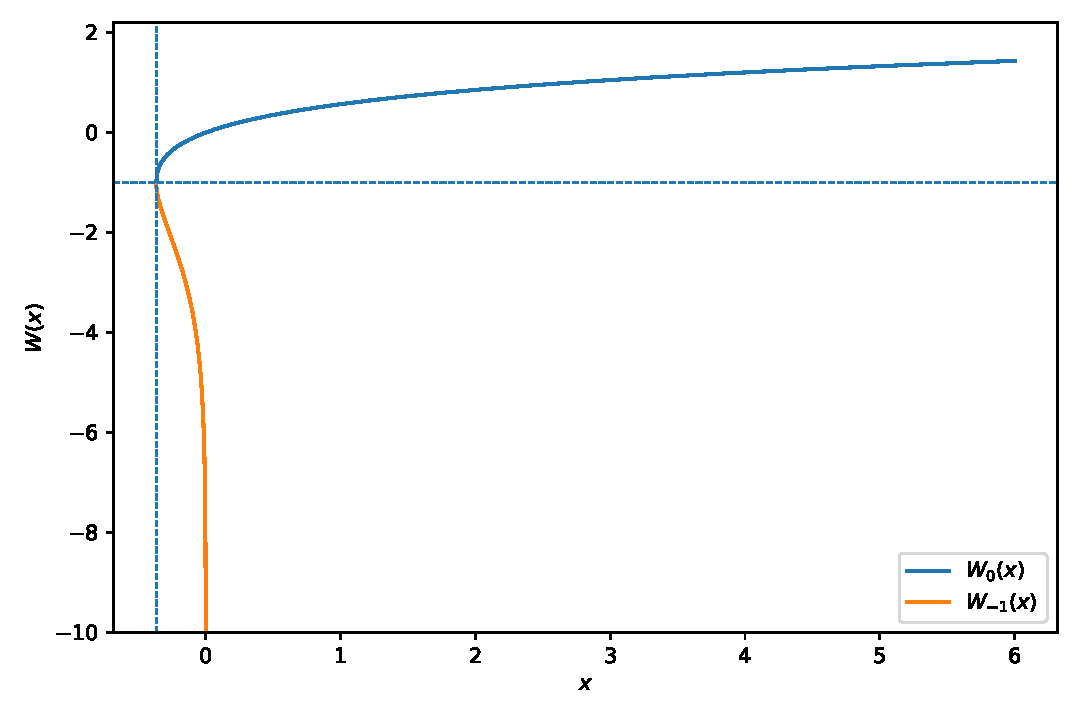
\includegraphics[width=0.82\textwidth]{real_branches.pdf}
\caption{The two real branches.  The principal branch is increasing; the lower
branch is decreasing and tends to \(-\infty\) as \(x\to0^-\).}
\label{fig:realbranches}
\end{figure}

\begin{remark}[The nonprincipal real branch is not secondary]
Many expositions introduce \(\Wmone\) as an afterthought.  This is a mistake in
applications.  Whenever an equation has two admissible real solutions, the
second one is usually carried by \(\Wmone\).  Examples include \(x^x=a\) for a
range of \(a\), threshold equations, escape-time equations, delay spectra, and
asymptotic inversion in prime-number theory.
\end{remark}

\section{Basic values and limits}
The defining equation immediately gives a large family of exact values.

\begin{proposition}[Values generated from the inverse relation]\label{prop:exactvalues}
For every real \(a\ge -1\),
\[
       \Wzero(a\e^a)=a.
\]
For every real \(a\le -1\),
\[
       \Wmone(a\e^a)=a.
\]
In particular,
\[
\Wzero(0)=0,\qquad
\Wzero(-1/\e)=\Wmone(-1/\e)=-1,\qquad
\Wzero(\e)=1.
\]
Moreover,
\[
 \lim_{x\to\infty}\Wzero(x)=\infty,
 \qquad
 \lim_{x\to0^-}\Wmone(x)=-\infty.
\]
\end{proposition}

\begin{proof}
If \(x=a\e^a\), then \(a\) is a solution of \(w\e^w=x\).  The range
conditions in \Cref{thm:realbranches} select the branch.  The limits follow by
inverting the endpoint limits of \(f\) on the corresponding monotonicity
intervals.
\end{proof}

The number
\[
      \Omega=\Wzero(1)=0.567143290409783872999968\ldots
\]
is called the \emph{omega constant}.  It is the unique positive solution of
\(\Omega\e^\Omega=1\), equivalently \(\Omega=\e^{-\Omega}\).

\begin{table}[htbp]
\centering
\caption{Representative real values, generated by the included Python program.}
\label{tab:values}
\begin{tabular}{@{}rcr@{}}
\toprule
argument & branch & value \\
\midrule
$-1/e$ & $W_0$ & $-1.0$ \\
$-1/e$ & $W_{-1}$ & $-1.0$ \\
$-0.35$ & $W_0$ & $-0.716638816456074$ \\
$-0.35$ & $W_{-1}$ & $-1.34971725219225$ \\
$-0.1$ & $W_0$ & $-0.111832559158963$ \\
$-0.1$ & $W_{-1}$ & $-3.5771520639573$ \\
$-10^{-6}$ & $W_0$ & $-1.0000010000015e-6$ \\
$-10^{-6}$ & $W_{-1}$ & $-16.6265089013725$ \\
$0$ & $W_0$ & $0.0$ \\
$0.1$ & $W_0$ & $0.0912765271608623$ \\
$1$ & $W_0$ & $0.567143290409784$ \\
$e$ & $W_0$ & $1.0$ \\
$10$ & $W_0$ & $1.7455280027407$ \\
$10^6$ & $W_0$ & $11.3833580861401$ \\
\bottomrule
\end{tabular}

\end{table}

\section{Complex branches in one page}\label{sec:complexbranches}
The function \(f(w)=w\e^w\) is entire.  Its derivative vanishes only at
\(w=-1\), so every local inverse is analytic except where continuation meets the
critical value \(-1/\e\), or where the inverse escapes to infinity.  The latter
phenomenon occurs at \(z=0\) on every nonprincipal branch.

A standard branch convention labels the infinitely many solutions so that, for
large \(z\),
\[
       W_k(z)\approx \Log z+2\pi\ii k
       -\Log\bigl(\Log z+2\pi\ii k\bigr).
\]
This formula explains the integer branch index: changing \(k\) changes the
logarithm by one turn around the origin.  The principal branch \(W_0\) is analytic
at \(0\), whereas \(W_k\) for \(k\ne0\) has logarithmic divergence there.  The
point \(-1/\e\) is a square-root branch point joining \(W_0\) to \(W_{-1}\).
Detailed cut conventions are discussed in the canonical paper of Corless et
al.~\cite{Corless1996}; for real-variable work, \Cref{thm:realbranches} removes
all ambiguity.

\chapter{Calculus of \texorpdfstring{\(W_0\)}{W0} and
\texorpdfstring{\(W_{-1}\)}{W-1}}\label{chap:calculus}

\section{First derivative and monotonicity}
Let \(W\) denote any differentiable branch at a point where
\(W\ne-1\).  Differentiate \(W(x)\e^{W(x)}=x\):
\[
   W'(x)\e^{W(x)}\bigl(1+W(x)\bigr)=1.
\]

\begin{theorem}[Derivative formulas]\label{thm:derivative}
At every regular point of a branch,
\begin{align}
 W'(x)
 &=\frac{\e^{-W(x)}}{1+W(x)},\label{eq:derivative1}\\
 &=\frac{W(x)}{x\bigl(1+W(x)\bigr)},\qquad x\ne0.\label{eq:derivative2}
\end{align}
For the principal branch, \(\Wzero'(0)=1\).
\end{theorem}

\begin{proof}
The first formula follows from implicit differentiation.  For \(x\ne0\), the
identity \(\e^{-W}=W/x\), obtained from \(W\e^W=x\), gives the second formula.
At the origin, \(f'(0)=1\), so the inverse function theorem gives
\(\Wzero'(0)=1/f'(0)=1\).  Equivalently, take the limit in
\eqref{eq:derivative1}.
\end{proof}

The signs now agree with the geometric argument:
\[
 \Wzero'(x)>0\quad(x>-1/\e),
 \qquad
 \Wmone'(x)<0\quad(-1/\e<x<0).
\]
Both derivatives become unbounded in magnitude at the branch point.

\section{Second derivative and curvature}
Differentiating \eqref{eq:derivative1} once more gives
\begin{equation}\label{eq:secondderivative}
 W''(x)=-\frac{\e^{-2W(x)}\bigl(W(x)+2\bigr)}
                   {\bigl(1+W(x)\bigr)^3}.
\end{equation}

\begin{theorem}[Concavity and the inflection point of \(W_{-1}\)]
The principal branch \(\Wzero\) is strictly concave on
\((-1/\e,\infty)\).  The branch \(\Wmone\) is strictly convex on
\[
   \left(-\frac1\e,-\frac{2}{\e^2}\right)
\]
and strictly concave on
\[
   \left(-\frac{2}{\e^2},0\right).
\]
Its unique inflection point is
\[
      \left(-\frac{2}{\e^2},-2\right).
\]
\end{theorem}

\begin{proof}
On \(W_0\), one has \(W>-1\), so the denominator in
\eqref{eq:secondderivative} is positive, while \(W+2>1\).  Hence
\(W_0''<0\).

On \(W_{-1}\), the denominator is negative.  Therefore the sign of \(W''\)
is the sign of \(W+2\): it is positive when \(-2<W<-1\), zero at
\(W=-2\), and negative when \(W<-2\).  The corresponding argument at
\(W=-2\) is \(-2\e^{-2}\).  Since \(W_{-1}\) is decreasing, the stated
interval order follows.
\end{proof}

\section{Higher derivatives}
Repeated differentiation has a useful uniform structure.

\begin{theorem}[Derivative polynomials]\label{thm:derivativepolynomials}
Define polynomials \(P_n\) by
\[
 P_1(w)=1,
 \qquad
 P_{n+1}(w)=(1+w)P_n'(w)-(nw+3n-1)P_n(w).
\]
Then, for \(n\ge1\),
\begin{equation}\label{eq:nthderivative}
   \frac{\dd^n}{\dd x^n}W(x)
   =\frac{\e^{-nW(x)}P_n(W(x))}
          {(1+W(x))^{2n-1}}.
\end{equation}
The first polynomials are
\[
 P_1=1,\quad P_2=-(w+2),\quad
 P_3=2w^2+8w+9,
\]
\[
 P_4=-(6w^3+36w^2+79w+64).
\]
At the origin,
\[
       P_n(0)=\Wzero^{(n)}(0)=(-n)^{n-1}.
\]
\end{theorem}

\begin{proof}
The case \(n=1\) is \eqref{eq:derivative1}.  Assume
\eqref{eq:nthderivative}.  Since
\[
   \frac{\dd}{\dd x}=\frac{\e^{-W}}{1+W}\frac{\dd}{\dd W},
\]
we obtain
\begin{align*}
 \frac{\dd^{n+1}W}{\dd x^{n+1}}
 &=\frac{\e^{-W}}{1+W}\frac{\dd}{\dd W}
   \left(\e^{-nW}P_n(W)(1+W)^{-(2n-1)}\right)\\
 &=\frac{\e^{-(n+1)W}}{(1+W)^{2n+1}}
   \left((1+W)P_n'(W)-(nW+3n-1)P_n(W)\right),
\end{align*}
which is the required recurrence.  The displayed polynomials follow by direct
calculation.  The value at zero will also follow from the Taylor series in
\Cref{thm:maclaurin}; alternatively, the recurrence at \(w=0\) proves it by
induction after the same coefficient identity is established.
\end{proof}

\section{Differential equations}
The derivative identity can be written without exponentials:
\begin{equation}\label{eq:firstode}
       x(1+W)W'=W.
\end{equation}
Thus every scaled function \(w(x)=W(cx)\) solves the same first-order nonlinear
differential equation.  Differentiating \eqref{eq:firstode} gives a second-order
equation,
\begin{equation}\label{eq:secondode}
 x(1+W)W''+x(W')^2+W W'=0.
\end{equation}
These identities are often more convenient than the original inverse relation in
symbolic calculations.

\section{Conditioning}\label{sec:conditioning}
If the input \(x\) is perturbed by a small relative amount, the first-order
relative response of \(W\) is measured by
\[
  \kappa_W(x)=\abs{\frac{xW'(x)}{W(x)}}.
\]
Using \eqref{eq:derivative2} gives an unusually simple answer.

\begin{proposition}[Relative condition number]\label{prop:condition}
For either real branch away from the branch point and from the removable point
\(x=0\) of \(W_0\),
\[
       \kappa_W(x)=\frac1{\abs{1+W(x)}}.
\]
Near \(-1/\e\),
\[
       \kappa_W(x)\sim \frac1{\sqrt{2(1+\e x)}}.
\]
This holds after choosing either real branch.
\end{proposition}

\begin{proof}
The exact formula follows immediately from \eqref{eq:derivative2}.  The
branch-point expansion in \Cref{thm:puiseux} gives
\(1+W_0\sim p\) and \(1+W_{-1}\sim-p\), where
\(p=\sqrt{2(1+\e x)}\).  Taking absolute values gives the asymptotic form.
\end{proof}

\begin{figure}[htbp]
\centering
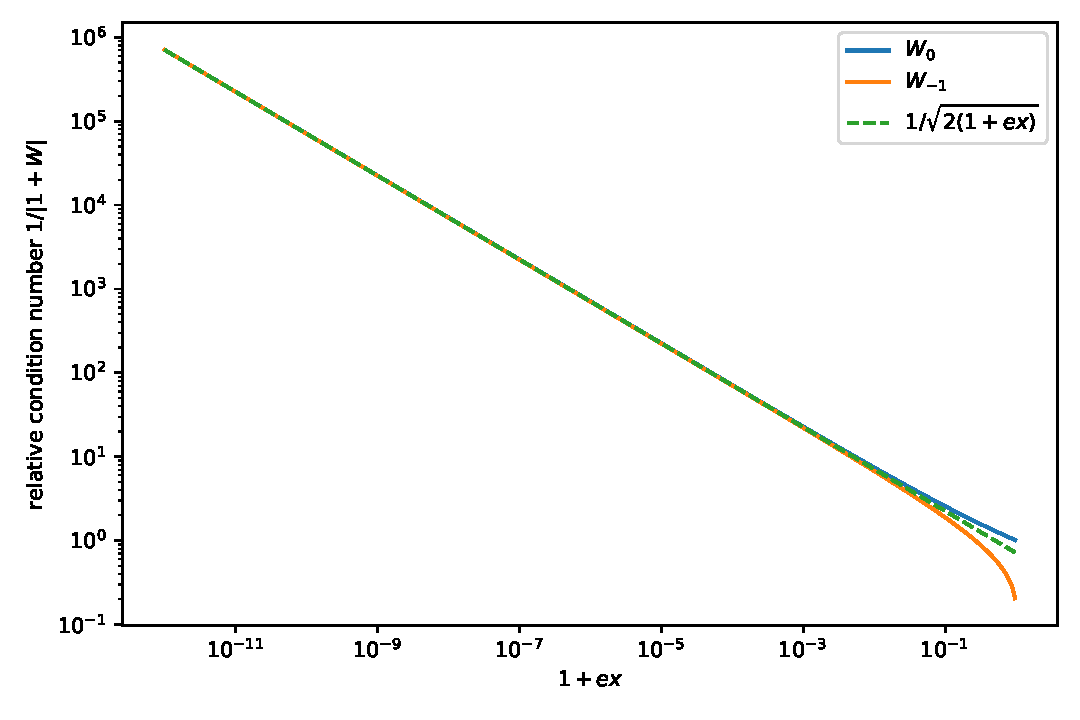
\includegraphics[width=0.82\textwidth]{conditioning.pdf}
\caption{Relative conditioning of both real branches near the branch point.
The square-root blow-up is the principal numerical difficulty of the problem.}
\label{fig:conditioning}
\end{figure}

\chapter{Solving equations with Lambert \texorpdfstring{\(W\)}{W}}\label{chap:equations}

\section{A disciplined reduction method}
The usual goal is to transform an equation until the unknown occurs in a product
of the form
\[
       u\e^u=c.
\]
Then \(u=W_k(c)\).  The algebra is generally easy; branch selection is the
substantive step.

\begin{proposition}[Affine exponential equation]\label{prop:affineexp}
Let \(a,c\ne0\).  Every solution of
\[
       \e^{ax+b}=cx+d
\]
is of the form
\begin{equation}\label{eq:affineexpsolution}
 x=-\frac1a W_k\!\left(-\frac{a}{c}
        \exp\!\left(b-\frac{ad}{c}\right)\right)-\frac dc,
\end{equation}
for a branch \(k\) on which the expression is defined.
\end{proposition}

\begin{proof}
Set \(y=cx+d\), so \(x=(y-d)/c\).  The equation becomes
\[
  \exp\!\left(\frac ac y+b-\frac{ad}{c}\right)=y.
\]
Multiplying by \(\exp(-ay/c)\) and then by \(-a/c\) yields
\[
  \left(-\frac ac y\right)
  \exp\!\left(-\frac ac y\right)
  =-\frac ac\exp\!\left(b-\frac{ad}{c}\right).
\]
Apply \(W_k\), solve for \(y\), and then for \(x\).
\end{proof}

\begin{example}
The equation \(2^x=x+3\) has the form of \Cref{prop:affineexp} with
\(a=\log2\), \(b=0\), \(c=1\), and \(d=3\).  Therefore
\[
 x=-\frac{1}{\log2}W_k\!\left(-\log2\,2^{-3}\right)-3.
\]
Because the argument lies in \((-1/\e,0)\), two real branches are available.
The original equation or a graph determines whether both values satisfy the
problem's constraints.
\end{example}

\section{Powers times exponentials}

\begin{proposition}\label{prop:powerexp}
Suppose \(m\in\mathbb N\), \(q\ne0\), and a real \(m\)-th root \(r^{1/m}\) has been
chosen consistently.  Solutions of
\[
       x^m\e^{qx}=r
\]
that correspond to this root satisfy
\[
       x=\frac mq W_k\!\left(\frac qm r^{1/m}\right).
\]
\end{proposition}

\begin{proof}
Taking the selected \(m\)-th root gives
\(x\e^{qx/m}=r^{1/m}\).  Multiply by \(q/m\) and apply \(W_k\).
For even \(m\), the other real root may produce additional solutions and must be
examined separately.
\end{proof}

\section{The equations \texorpdfstring{\(x\log x=a\)}{x log x=a} and
\texorpdfstring{\(x^x=a\)}{x to the x = a}}

\begin{proposition}\label{prop:xlogx}
For \(x>0\), the equation \(x\log x=a\) is solved by
\[
       x=\exp(W_k(a))=\frac{a}{W_k(a)},
\]
with the quotient interpreted by continuity at \(a=0\).
\end{proposition}

\begin{proof}
Set \(u=\log x\), so \(x=\e^u\).  Then
\(x\log x=u\e^u=a\), hence \(u=W_k(a)\), and exponentiation gives the result.
The identity \(\e^{W(a)}=a/W(a)\) follows from the defining equation.
\end{proof}

\begin{theorem}[Complete real analysis of \(x^x=a\)]\label{thm:xx}
For \(x>0\),
\[
       x^x=a
       \quad\Longleftrightarrow\quad
       x=\exp\bigl(W_k(\log a)\bigr).
\]
Let \(a_*=\e^{-1/\e}\).  Then:
\begin{enumerate}[label=(\alph*)]
\item if \(0<a<a_*\), there is no positive real solution;
\item if \(a=a_*\), there is one solution, \(x=1/\e\);
\item if \(a_*<a<1\), there are two solutions, obtained from \(W_0\) and
      \(W_{-1}\);
\item if \(a\ge1\), there is one positive solution, obtained from \(W_0\).
\end{enumerate}
\end{theorem}

\begin{proof}
Taking logarithms gives \(x\log x=\log a\), so \Cref{prop:xlogx} yields the
formula.  The function \(g(x)=x\log x\) has derivative \(1+\log x\), hence its
minimum occurs at \(x=1/\e\) and equals \(-1/\e\).  Equivalently,
\(x^x\) has minimum \(\e^{-1/\e}\).  The number of solutions on either side of
the minimum agrees exactly with the two real branches described in
\Cref{thm:realbranches}.
\end{proof}

\section{Infinite power towers}
The finite towers are defined recursively by
\[
       t_1=a,\qquad t_{n+1}=a^{t_n}\quad(n\ge1),
\]
where \(a>0\).  If \((t_n)\) converges to a positive limit \(h\), continuity
forces \(h=a^h\).  Solving this fixed-point equation gives a Lambert \(W\)
formula, but the existence of a fixed point does not by itself guarantee that
the iteration converges to it.

\begin{theorem}[Exact real power-tower interval]\label{thm:powertower}
The sequence of finite towers \((t_n)\) converges if and only if
\[
                 \e^{-\e}\le a\le \e^{1/\e}.
\]
Throughout this interval its limit is
\begin{equation}\label{eq:powertower}
 h=\begin{cases}
  -\dfrac{W_0(-\log a)}{\log a},&a\ne1,\\[8pt]
  1,&a=1.
 \end{cases}
\end{equation}
For \(1<a<\e^{1/\e}\), the second real branch \(W_{-1}\) produces another
positive solution of \(h=a^h\), but that solution is repelling and is not the
limit of the finite towers.
\end{theorem}

\begin{proof}
First solve the fixed-point equation.  For \(a\ne1\), taking logarithms in
\(h=a^h\) and putting \(u=-h\log a\) gives
\[
             u\e^u=-\log a,
\]
hence
\[
             h=-\frac{W_k(-\log a)}{\log a}.
\]
For \(a=1\), every finite tower equals \(1\), and the value in
\eqref{eq:powertower} is also obtained by continuity.

It remains to decide when the iteration converges.  Write
\(g(x)=a^x\), so that \(t_{n+1}=g(t_n)\).  At a fixed point,
\[
       g'(h)=h\log a=\log h=-W_k(-\log a).
\]
Thus a locally attracting fixed point must satisfy \(\abs{\log h}<1\), or
\(1/\e<h<\e\).  The endpoints will be handled directly below.

Suppose first that \(1<a\le\e^{1/\e}\).  The function
\(q(h)=h^{1/h}\) increases on \([1,\e]\), because
\[
       \frac{q'(h)}{q(h)}=\frac{1-\log h}{h^2}\ge0.
\]
Consequently there is a unique \(h\in[1,\e]\) such that \(a=q(h)\), and this
is precisely the value obtained from \(W_0\).  Since
\(a=h^{1/h}\le h\), the first term satisfies \(t_1\le h\).  Moreover,
\(g\) is increasing, \(t_2=a^a\ge a=t_1\), and
\(g([t_1,h])\subseteq[t_1,h]\).  Induction therefore shows that \((t_n)\) is
increasing and bounded above by \(h\).  Its limit must be a fixed point and
hence equals \(h\).  This argument includes the neutral upper endpoint
\(a=\e^{1/\e}\), where \(h=\e\) and \(g'(h)=1\).

Now suppose that \(\e^{-\e}\le a<1\), and write \(a=\e^{-A}\), so
\(0<A\le\e\).  There is a unique fixed point \(h\in[1/\e,1)\), again given
by \(W_0\).  Since \(a=h^{1/h}<h\) and \(g\) is decreasing,
\[
        t_1<h<t_2.
\]
Also every term lies in \((0,1)\).  The odd subsequence is increasing and the
even subsequence is decreasing: indeed \(t_3=a^{t_2}>a=t_1\), because
\(t_2<1\), and then the monotonicity of \(g\circ g\) propagates these
inequalities.  Both subsequences are bounded by \(h\), so they have limits
\(p\le h\le q\) satisfying
\[
                 p=g(q),\qquad q=g(p).
\]
We show that \(p=q\).  Otherwise \(0<p<q<1\) would be a nontrivial two-cycle.
Put \(u=-\log p\) and \(v=-\log q\), so \(u>v>0\).  The two-cycle equations
give
\[
                 A=u\e^v=v\e^u,
\]
and therefore \(\log(u/v)=u-v\).  Writing \(r=u/v>1\), we obtain
\[
 v=\frac{\log r}{r-1},\qquad
 u=\frac{r\log r}{r-1},\qquad
 A=\frac{r\log r}{r-1}\,r^{1/(r-1)}.
\]
This last quantity is strictly larger than \(\e\).  To see this, put
\(r=\e^s\), \(s>0\), and let \(F(s)\) be its logarithm.  Direct
differentiation gives
\[
 F'(s)=
 \frac{(\e^s-1)^2-s^2\e^s}
      {s(\e^s-1)^2}>0,
\]
because \(\e^s-1>s\e^{s/2}\), which is equivalent to
\(2\sinh(s/2)>s\).  Since \(F(s)\to1\) as \(s\downarrow0\), we have
\(A>\e\), contradicting \(A\le\e\).  Hence \(p=q=h\), and the full sequence
converges.  This includes the neutral lower endpoint \(a=\e^{-\e}\), where
\(h=1/\e\) and \(g'(h)=-1\).

Finally, if \(a>\e^{1/\e}\), then \(h^{1/h}=a\) has no positive solution,
because \(q\) has global maximum \(q(\e)=\e^{1/\e}\).  If
\(0<a<\e^{-\e}\), its unique fixed point lies below \(1/\e\) and satisfies
\(\abs{g'(h)}=\abs{\log h}>1\).  Were the distinct iterates to converge to
\(h\), the mean value theorem would eventually expand, rather than shrink,
their distance from \(h\).  They cannot land on \(h\) in finitely many steps:
since \(g\) is one-to-one, that would force every preceding term, including
\(t_1=a\), to equal \(h\), which is impossible for \(0<a<1\).  Thus no
convergence occurs outside the stated interval.

For \(1<a<\e^{1/\e}\), the \(W_{-1}\) value corresponds to a second fixed
point \(H>\e\).  There \(g'(H)=\log H>1\), so it is repelling.  The finite
towers instead converge to the attracting \(W_0\) fixed point in \((1,\e)\).
\end{proof}

\section{A branch-selection checklist}
For a real problem, the following short procedure prevents most mistakes.
\begin{enumerate}[label=\arabic*.]
\item Determine the transformed argument \(z\).
\item If \(z<-1/\e\), no real \(W\)-value exists.
\item If \(-1/\e<z<0\), write down both \(W_0(z)\) and \(W_{-1}(z)\).
\item Translate the ranges \([-1,0)\) and \(( -\infty,-1]\) back to the
      original variable.
\item Check every surviving candidate in the original equation, especially if
      roots or logarithms were introduced.
\end{enumerate}


\part{Series, local structure, and asymptotics}

\chapter{Power series and Lagrange inversion}\label{chap:taylor}

\section{Coefficient extraction and the inversion theorem}
Power series are the natural language of a locally analytic inverse.  We use
\([z^n]F(z)\) to denote the coefficient of \(z^n\) in a power series \(F\).
The following form of the Lagrange--B\"urmann inversion theorem is sufficient
for almost everything in this chapter.

\begin{theorem}[Lagrange--B\"urmann inversion]\label{thm:lagrange}
Let \(\phi\) be analytic near \(0\), with \(\phi(0)\ne0\), and let \(w(z)\)
be the analytic solution near the origin of
\[
             w=z\phi(w),\qquad w(0)=0.
\]
If \(F\) is analytic near \(0\), then for every integer \(n\ge1\),
\begin{equation}\label{eq:lagrange}
 [z^n]F(w(z))=\frac1n[t^{n-1}]F'(t)\phi(t)^n.
\end{equation}
In particular,
\[
 [z^n]w(z)^m=\frac mn[t^{n-m}]\phi(t)^n
 \qquad(n\ge m\ge1).
\]
\end{theorem}

\begin{proof}
Choose small positively oriented circles on which all functions involved are
analytic and on which the substitution \(t=w(z)\) is one-to-one.  Since
\(z=t/\phi(t)\), Cauchy's coefficient formula and a change of variable give
\begin{align*}
 [z^n]F(w(z))
 &=\frac{1}{2\pi\ii}\int
       \frac{F(w(z))}{z^{n+1}}\dd z\\
 &=\frac{1}{2\pi\ii}\int
   F(t)\left(
      \frac{\phi(t)^n}{t^{n+1}}
      -\frac{\phi(t)^{n-1}\phi'(t)}{t^n}
   \right)\dd t.
\end{align*}
The integrand satisfies the exact identity
\[
 F(t)\left(
      \frac{\phi(t)^n}{t^{n+1}}
      -\frac{\phi(t)^{n-1}\phi'(t)}{t^n}
   \right)
 =-\frac1n\frac{\dd}{\dd t}
   \left(\frac{F(t)\phi(t)^n}{t^n}\right)
  +\frac1n\frac{F'(t)\phi(t)^n}{t^n}.
\]
The integral of the total derivative around the closed contour is zero.
Equivalently, a derivative has residue zero.  Therefore
\[
 [z^n]F(w(z))
 =\frac{1}{2\pi\ii}\int
   \frac{F'(t)\phi(t)^n}{n t^n}\dd t
 =\frac1n[t^{n-1}]F'(t)\phi(t)^n.
\]
Taking \(F(t)=t^m\) proves the last assertion.
\end{proof}

\begin{remark}
The proof used complex integration only as a compact bookkeeping device.  The
identity is equally valid for formal power series, where it can be proved by
coefficient manipulations.  Thus it may be used before any questions about
numerical convergence are considered.
\end{remark}

\section{The Maclaurin series of the principal branch}
The relation \(w\e^w=z\) can be written
\[
             w=z\e^{-w}.
\]
Thus \(\phi(t)=\e^{-t}\) in \Cref{thm:lagrange}.

\begin{theorem}[Maclaurin series]\label{thm:maclaurin}
For \(\abs z<1/\e\),
\begin{equation}\label{eq:maclaurin}
 \Wzero(z)=\sum_{n=1}^{\infty}
       \frac{(-n)^{n-1}}{n!}z^n
 =z-z^2+\frac32z^3-\frac83z^4
  +\frac{125}{24}z^5-\cdots.
\end{equation}
The radius of convergence is exactly \(1/\e\).  The series also converges
absolutely at both endpoints \(z=\pm1/\e\), and at the negative endpoint its
sum is \(-1\).
\end{theorem}

\begin{proof}
Apply \Cref{thm:lagrange} with \(F(t)=t\):
\[
 [z^n]\Wzero(z)
 =\frac1n[t^{n-1}]\e^{-nt}
 =\frac1n\frac{(-n)^{n-1}}{(n-1)!}
 =\frac{(-n)^{n-1}}{n!}.
\]
Stirling's formula gives
\[
 \frac{n^{n-1}}{n!}
 \sim\frac{\e^n}{\sqrt{2\pi}\,n^{3/2}},
\]
so the root test gives radius \(1/\e\).  This radius is also geometrically
inevitable: the nearest point at which the inverse ceases to be locally
analytic is the critical value \(-1/\e\).

At \(z=\pm1/\e\), the absolute values of the terms are asymptotic to
\(1/(\sqrt{2\pi}n^{3/2})\), so both endpoint series converge absolutely.  On
\((-1/\e,0)\) the sum is the analytic inverse \(W_0\); continuity up to the
endpoint, or Abel's theorem, then gives the value \(W_0(-1/\e)=-1\).
\end{proof}

\begin{warning}
The series \eqref{eq:maclaurin} belongs to \(W_0\), not to \(W_{-1}\).  The
lower real branch diverges to \(-\infty\) as \(x\to0^-\), so it cannot possess
a Taylor series at the origin.  Its appropriate local expansion is logarithmic
and is developed in \Cref{sec:wm1asymp}.
\end{warning}

\section{Powers and exponentials of \texorpdfstring{\(W_0\)}{W0}}
The full strength of Lagrange inversion gives many related series at almost no
additional cost.

\begin{proposition}[Powers of \(W_0\)]\label{prop:wpowerseries}
For every integer \(m\ge1\),
\begin{equation}\label{eq:wpowerseries}
 \Wzero(z)^m
 =\sum_{n=m}^{\infty}
   \frac{m}{n}\frac{(-n)^{n-m}}{(n-m)!}z^n,
 \qquad \abs z<1/\e.
\end{equation}
\end{proposition}

\begin{proof}
Use \(F(t)=t^m\) and \(\phi(t)=\e^{-t}\) in
\Cref{thm:lagrange}:
\[
 [z^n]W_0(z)^m
 =\frac mn[t^{n-m}]\e^{-nt}
 =\frac mn\frac{(-n)^{n-m}}{(n-m)!}.
\]
\end{proof}

\begin{proposition}[Exponentials of \(W_0\)]\label{prop:expwseries}
For every complex parameter \(a\),
\begin{equation}\label{eq:expwseries}
 \exp\!\bigl(a\Wzero(z)\bigr)
 =1+\sum_{n=1}^{\infty}
   \frac{a(a-n)^{n-1}}{n!}z^n,
 \qquad \abs z<1/\e.
\end{equation}
The formula is interpreted by continuity when \(a=0\).
\end{proposition}

\begin{proof}
For \(F(t)=\e^{at}\), \Cref{thm:lagrange} gives
\[
 [z^n]\e^{aW_0(z)}
 =\frac an[t^{n-1}]\e^{(a-n)t}
 =\frac{a(a-n)^{n-1}}{n!}.
\]
The constant term is \(1\).
\end{proof}

Setting \(a=-1\), for example, gives a series for
\(\e^{-W_0(z)}=W_0(z)/z\).  Differentiating \eqref{eq:maclaurin} gives
series for \(W_0'\) and, through
\(zW_0'=W_0/(1+W_0)\), for rational expressions in \(W_0\).

\section{Taylor series about an arbitrary regular point}
The origin is not privileged.  Let \(w_*\ne-1\), put
\(z_*=w_*\e^{w_*}\), and choose the local inverse branch satisfying
\(W(z_*)=w_*\).  Taylor's theorem and the derivative formulas of
\Cref{chap:calculus} give
\begin{align}
 W(z_*+\Delta)
 ={}&w_*+\frac{\e^{-w_*}}{1+w_*}\Delta
 -\frac{\e^{-2w_*}(w_*+2)}{2(1+w_*)^3}\Delta^2\notag\\
 &+\frac{\e^{-3w_*}(2w_*^2+8w_*+9)}{6(1+w_*)^5}\Delta^3
 +\bigO(\Delta^4).
\label{eq:inversetaylor}
\end{align}
This expansion is valid on either real branch.  The coefficients become large
as \(w_*\to-1\), signaling that an ordinary Taylor series is the wrong local
coordinate at the branch point.  Formula \eqref{eq:inversetaylor} is also the
basis of the Schr\"oder-type corrections in \Cref{sec:schroeder}.

\begin{theorem}[Local inverse series on both real branches]
Let \(w_*\in(-\infty,-1)\cup(-1,\infty)\), and
\(z_*=w_*\e^{w_*}\).  Then there is a disk centered at \(z_*\) on which a
unique analytic inverse branch satisfies \(W(z_*)=w_*\), and its Taylor
coefficients are \(W^{(n)}(z_*)/n!\), with \(W^{(n)}\) given by
\eqref{eq:nthderivative}.
\end{theorem}

\begin{proof}
The derivative of \(f(w)=w\e^w\) at \(w_*\) is
\(\e^{w_*}(1+w_*)\ne0\).  The analytic inverse function theorem therefore
produces a unique analytic local inverse.  Taylor's theorem supplies the
series, and \Cref{thm:derivativepolynomials} supplies every coefficient.
\end{proof}

\section{The tree function}
The sign change
\[
             T(z)=-\Wzero(-z)
\]
produces the classical tree function.  From \eqref{eq:maclaurin},
\begin{equation}\label{eq:treeseries}
       T(z)=\sum_{n=1}^{\infty}\frac{n^{n-1}}{n!}z^n,
       \qquad \abs z<1/\e,
\end{equation}
and the defining relation is
\[
             T(z)\e^{-T(z)}=z,
             \qquad T(z)=z\e^{T(z)}.
\]
The coefficient \(n^{n-1}\) counts rooted labeled trees on \(n\) vertices.
A complete combinatorial explanation is given in \Cref{chap:trees}.

\chapter{The square-root branch point}\label{chap:branchpoint}

\section{Why ordinary Taylor series fail}
At \(w=-1\), the derivative of \(f(w)=w\e^w\) vanishes, while
\(f''(-1)=\e^{-1}\ne0\).  Thus the graph has a nondegenerate quadratic
turning point.  Inverting a quadratic relation produces a square root, so the
correct local series is a Puiseux series, a power series in a square-root
variable.

Write
\[
       w=-1+u,
       \qquad
       p=\sqrt{2(1+\e x)}.
\]
Then
\begin{equation}\label{eq:pueq}
 \frac{p^2}{2}=1+(-1+u)\e^u
 =\frac{u^2}{2}+\frac{u^3}{3}
   +\frac{u^4}{8}+\frac{u^5}{30}+\cdots.
\end{equation}
The principal square root gives \(p\ge0\) for real
\(x\ge-1/\e\).

\section{An all-order coefficient formula}
Define the analytic function
\begin{equation}\label{eq:phibranch}
 \Phi(u)=
 \left(\frac{2\{1+(-1+u)\e^u\}}{u^2}\right)^{1/2},
 \qquad \Phi(0)=1.
\end{equation}
Equation \eqref{eq:pueq} is \(p=u\Phi(u)\), or
\(u=p/\Phi(u)\).  Lagrange inversion applies once more.

\begin{theorem}[Puiseux expansion at \(-1/\e\)]\label{thm:puiseux}
There is a convergent power series
\[
             U(p)=\sum_{n=1}^{\infty}c_np^n
\]
near \(p=0\), where
\begin{equation}\label{eq:branchcoeff}
 c_n=\frac1n[t^{n-1}]\Phi(t)^{-n},
\end{equation}
with \(\Phi\) defined by \eqref{eq:phibranch}.  The two real branches are
obtained from the same series by
\begin{align}
 \Wzero(x)&=-1+U(p),\label{eq:w0branchseries}\\
 \Wmone(x)&=-1+U(-p),\label{eq:wm1branchseries}
\end{align}
where \(p=\sqrt{2(1+\e x)}\).  The first terms are
\begin{align}
 U(p)={}&p-\frac13p^2+\frac{11}{72}p^3
 -\frac{43}{540}p^4+\frac{769}{17280}p^5
 -\frac{221}{8505}p^6\notag\\
 &+\frac{680863}{43545600}p^7
 -\frac{1963}{204120}p^8
 +\frac{226287557}{37623398400}p^9
 -\frac{5776369}{1515591000}p^{10}+\bigO(p^{11}).
\label{eq:Ucoefficients}
\end{align}
\end{theorem}

\begin{proof}
The quotient inside \(\Phi\) has a removable singularity at the origin and
has value \(1\) there, as follows from \eqref{eq:pueq}.  Hence \(\Phi\) is
analytic and nonzero near \(0\).  The analytic inverse function theorem gives
a unique analytic solution \(u=U(p)\) of \(p=u\Phi(u)\), with \(U(0)=0\) and
\(U'(0)=1\).  Applying \Cref{thm:lagrange} to
\(u=p\Phi(u)^{-1}\) yields \eqref{eq:branchcoeff}.  Substitution and
coefficient comparison give the displayed rational numbers.

For real \(x>-1/\e\), the solution with \(u>0\) belongs to the range
\((-1,\infty)\) and is therefore \(W_0\); this is \(U(p)\).  The solution
with \(u<0\) is obtained by choosing the other sign of the square root, hence
by replacing \(p\) by \(-p\).  On the real interval where it exists, this is
\(W_{-1}\).  This proves both branch formulas.
\end{proof}

\begin{corollary}[Leading branch-point behavior]\label{cor:branchlead}
As \(x\downarrow-1/\e\), with \(p=\sqrt{2(1+\e x)}\),
\begin{align*}
 \Wzero(x)&=-1+p-\frac13p^2+\bigO(p^3),\\
 \Wmone(x)&=-1-p-\frac13p^2+\bigO(p^3).
\end{align*}
Consequently,
\[
 W_0(x)-W_{-1}(x)=2p+\frac{11}{36}p^3+\bigO(p^5),
\]
and
\[
 W_0(x)+W_{-1}(x)=-2-\frac23p^2-\frac{43}{270}p^4+\bigO(p^6).
\]
\end{corollary}

\begin{proof}
Insert \(p\) and \(-p\) into \eqref{eq:Ucoefficients}.  Odd powers change
sign and even powers do not.  Addition and subtraction give the two final
formulas.
\end{proof}

\section{Derivatives and conditioning revisited}
Differentiating the leading terms, or using \Cref{thm:derivative}, gives
\begin{align*}
 W_0'(x)&\sim \frac{\e}{p},\\
 W_{-1}'(x)&\sim-\frac{\e}{p},
\end{align*}
where \(p=\sqrt{2(1+\e x)}\).  The two graphs therefore meet with vertical
opposite tangents.  No finite-order polynomial in \(x+1/\e\) can represent
this behavior; the square-root coordinate is essential.

\begin{figure}[htbp]
\centering
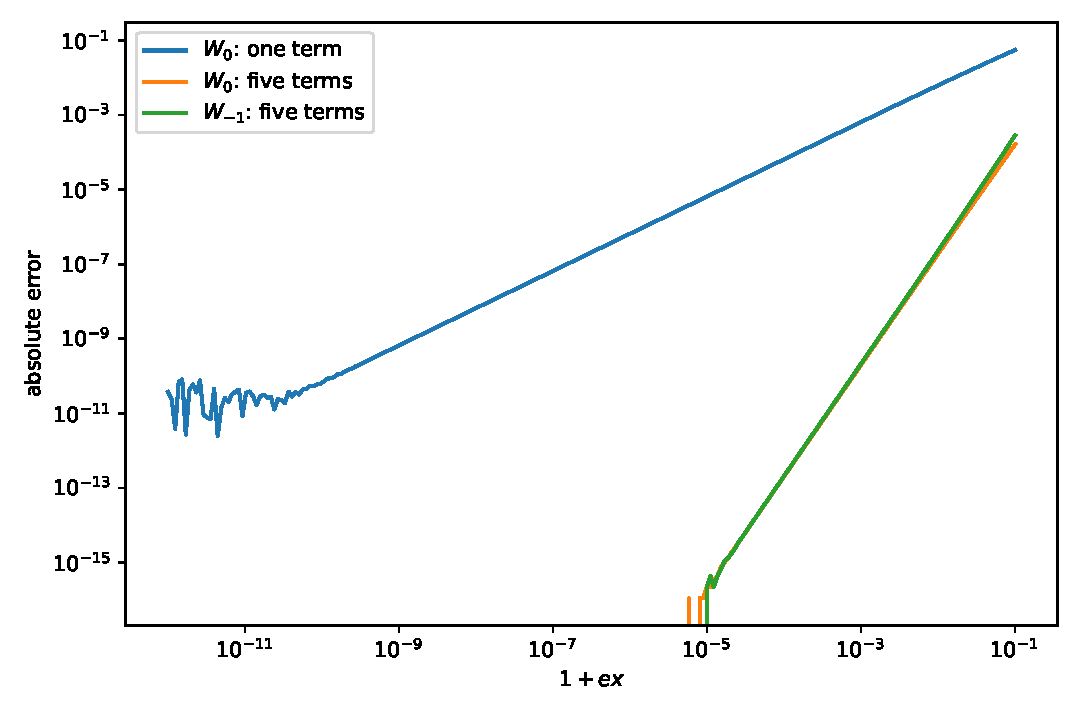
\includegraphics[width=0.82\textwidth]{branch_point_errors.pdf}
\caption{Errors of truncated Puiseux expansions as the branch point is
approached.  The same coefficient table serves both real branches.}
\label{fig:branchpointerrors}
\end{figure}

\section{A practical branch-point coordinate}
The exact identity
\[
              x=\frac{p^2/2-1}{\e}
\]
means that no further inversion is needed once \(p\) is known.  For numerical
work, the expression \(1+\e x\) can suffer cancellation when \(x\) is
extremely close to \(-1/\e\).  If the input itself is supplied as
\(x=-1/\e+\delta\), it is preferable to compute
\(p=\sqrt{2\e\delta}\) directly.  Likewise, if
\(x=-\e^{-1-u}\), then
\[
       p=\sqrt{2(1-\e^{-u})},
\]
which can be evaluated accurately with an \texttt{expm1}-type routine.

\chapter{Logarithmic asymptotic expansions}\label{chap:asymptotic}

\section{The universal asymptotic polynomials}
Large values of \(W\) are found by taking logarithms of the defining relation:
\begin{equation}\label{eq:logform}
              W+\Log W=\Log z,
\end{equation}
with compatible logarithm branches.  A family of polynomials organizes the
successive corrections.

\begin{definition}[Asymptotic polynomials]\label{def:Pn}
Let \(P_n(\ell)\) be determined recursively by
\begin{equation}\label{eq:Precurrence}
 P_n(\ell)=-[t^n]\log\left(
  1-\ell t+\sum_{j=1}^{n-1}P_j(\ell)t^{j+1}
 \right),\qquad n\ge1.
\end{equation}
Then
\begin{align*}
P_1(\ell)&=\ell,\\
P_2(\ell)&=\frac{\ell(\ell-2)}2,\\
P_3(\ell)&=\frac{\ell(2\ell^2-9\ell+6)}6,\\
P_4(\ell)&=\frac{\ell(3\ell^3-22\ell^2+36\ell-12)}{12},\\
P_5(\ell)&=\frac{\ell(12\ell^4-125\ell^3+350\ell^2-300\ell+60)}{60},\\
P_6(\ell)&=\frac{\ell(20\ell^5-274\ell^4+1125\ell^3-1700\ell^2
          +900\ell-120)}{120}.
\end{align*}
\end{definition}

The recurrence is constructive: to find \(P_n\), only the earlier polynomials
are required.  There is also a closed finite sum.  Let
\(\genfrac{[}{]}{0pt}{}{n}{j}\) denote an unsigned Stirling number of the first
kind.

\begin{proposition}[Stirling-number formula]\label{prop:Pstirling}
For \(n\ge1\),
\begin{equation}\label{eq:Pstirling}
 P_n(\ell)=\sum_{m=1}^{n}
   (-1)^{n-m}\genfrac{[}{]}{0pt}{}{n}{n-m+1}\frac{\ell^m}{m!}.
\end{equation}
\end{proposition}

\begin{proof}
The bivariate formal expansion
\begin{equation}\label{eq:doubleasymp}
 \sum_{r=0}^{\infty}\sum_{m=1}^{\infty}
   (-1)^r\genfrac{[}{]}{0pt}{}{r+m}{r+1}
   \frac{\ell^m}{m!}t^{r+m}
\end{equation}
solves, coefficient by coefficient, the equation
\[
 R(t)+\log\bigl(1-\ell t+tR(t)\bigr)=0,
 \qquad R(t)=\sum_{n\ge1}P_n(\ell)t^n.
\]
Indeed, the standard generating identity
\[
 \frac{(-\log(1-s))^{r+1}}{(r+1)!}
 =\sum_{n\ge r+1}\genfrac{[}{]}{0pt}{}{n}{r+1}\frac{s^n}{n!}
\]
reduces the coefficient verification to the power-series expansion of the
logarithm.  The coefficient of \(t^n\) in \eqref{eq:doubleasymp} is obtained
by setting \(r=n-m\), and is exactly \eqref{eq:Pstirling}.  Uniqueness of the
coefficient recursion \eqref{eq:Precurrence} completes the proof.
\end{proof}

\section{Large positive arguments on \texorpdfstring{\(W_0\)}{W0}}
Put
\[
             L=\log x,
             \qquad \ell=\log L.
\]
The first guess \(W_0(x)\approx L\) is improved by observing that
\(W+\log W=L\), so the next guess is \(L-\ell\).

\begin{theorem}[All-order expansion of \(W_0\)]\label{thm:w0asymp}
For every fixed integer \(N\ge0\), as \(x\to+\infty\),
\begin{equation}\label{eq:w0asymp}
 \Wzero(x)=L-\ell+\sum_{n=1}^{N}\frac{P_n(\ell)}{L^n}
 +\bigO\left(\frac{\ell^{N+1}}{L^{N+1}}\right),
\end{equation}
where an empty sum is understood when \(N=0\).  In particular,
\begin{align}
 W_0(x)={}&L-\ell+\frac{\ell}{L}
 +\frac{\ell(\ell-2)}{2L^2}
 +\frac{\ell(2\ell^2-9\ell+6)}{6L^3}\notag\\
 &+\frac{\ell(3\ell^3-22\ell^2+36\ell-12)}{12L^4}
 +\cdots.
\label{eq:w0asympexplicit}
\end{align}
\end{theorem}

\begin{proof}
Set \(t=1/L\) and seek
\[
 W=L-\ell+R,
 \qquad R=\sum_{n\ge1}P_n(\ell)t^n.
\]
Then
\[
 \log W=\ell+
 \log\left(1-\ell t+tR\right),
\]
so \(W+\log W-L=0\) becomes
\[
 R+\log(1-\ell t+tR)=0.
\]
Equating powers of \(t\) produces exactly \eqref{eq:Precurrence}, proving the
formal expansion.

For the asymptotic remainder, truncate after \(N\) terms and call the result
\(S_N\).  Direct substitution into \(F(w)=w+\log w-L\) gives
\[
 F(S_N)=\bigO\left(\frac{\ell^{N+1}}{L^{N+1}}\right).
\]
For large \(x\), both \(S_N\) and the exact root lie near \(L\), and
\(F'(w)=1+1/w\) is bounded away from zero.  The mean value theorem therefore
gives
\[
 W_0(x)-S_N=-\frac{F(S_N)}{F'(\xi)}
 =\bigO\left(\frac{\ell^{N+1}}{L^{N+1}}\right)
\]
for some \(\xi\) between \(S_N\) and \(W_0(x)\).
\end{proof}

\section{The lower branch near the origin}\label{sec:wm1asymp}
Let \(x\to0^-\), and define
\[
       T=\log\frac1{-x},
       \qquad \ell=\log T.
\]
Writing \(W_{-1}(x)=-u\), the defining equation becomes
\[
       u\e^{-u}=-x,
       \qquad u-\log u=T.
\]
The sign difference before \(\log u\) produces alternating signs in the
correction polynomials.

\begin{theorem}[All-order expansion of \(W_{-1}\)]\label{thm:wm1asymp}
For every fixed integer \(N\ge0\), as \(x\to0^-\),
\begin{equation}\label{eq:wm1asymp}
 \Wmone(x)=-T-\ell-
 \sum_{n=1}^{N}(-1)^{n-1}\frac{P_n(\ell)}{T^n}
 +\bigO\left(\frac{\ell^{N+1}}{T^{N+1}}\right).
\end{equation}
Thus
\begin{align}
 W_{-1}(x)={}&-T-\ell-\frac{\ell}{T}
 +\frac{\ell(\ell-2)}{2T^2}
 -\frac{\ell(2\ell^2-9\ell+6)}{6T^3}\notag\\
 &+\frac{\ell(3\ell^3-22\ell^2+36\ell-12)}{12T^4}
 +\cdots.
\label{eq:wm1asympexplicit}
\end{align}
\end{theorem}

\begin{proof}
Seek
\[
 u=T+\ell+\sum_{n\ge1}\frac{Q_n(\ell)}{T^n}.
\]
Substitution into \(u-\log u=T\), with \(t=1/T\), gives
\[
 Q-\log(1+\ell t+tQ)=0,
 \qquad Q=\sum_{n\ge1}Q_n(\ell)t^n.
\]
Replacing \(t\) by \(-t\) in the defining equation for the polynomials
\(P_n\) shows coefficient by coefficient that
\[
       Q_n(\ell)=(-1)^{n-1}P_n(\ell).
\]
Since \(W_{-1}=-u\), this gives the formal series
\eqref{eq:wm1asymp}.  The remainder proof is the same mean-value argument as
in \Cref{thm:w0asymp}, now applied to
\(G(u)=u-\log u-T\).  For large \(T\),
\(G'(u)=1-1/u\) is bounded away from zero.
\end{proof}

The leading two terms are often written directly in terms of \(x\):
\begin{equation}\label{eq:wm1twologs}
 W_{-1}(x)=\log(-x)-\log\bigl(-\log(-x)\bigr)+\littleo(1).
\end{equation}
This compact form is useful but converges slowly unless \(-x\) is extremely
small.

\section{Complex branches}\label{sec:complexasymp}
For a chosen branch index \(k\in\mathbb Z\), set
\[
 L_1=\Log z+2\pi\ii k,
 \qquad L_2=\Log L_1,
\]
with logarithms chosen consistently in the region under consideration.  The
same algebra used above gives the branch-uniform formal expansion
\begin{equation}\label{eq:complexasymp}
 W_k(z)\sim L_1-L_2+
       \sum_{n=1}^{\infty}\frac{P_n(L_2)}{L_1^n}.
\end{equation}
For fixed \(k\), it applies as \(z\to\infty\) away from the relevant cuts.  It
also describes \(W_k(z)\) as \(z\to0\) when \(k\ne0\), because then
\(\abs{L_1}\to\infty\).  This explains the logarithmic branch point of every
nonprincipal branch at the origin.

\begin{proof}[Derivation]
The logarithmic equation is
\(W+\Log W=L_1\).  Put
\(W=L_1-L_2+R\) and \(t=1/L_1\).  Exactly as in the proof of
\Cref{thm:w0asymp}, one obtains
\[
 R+\Log(1-L_2t+tR)=0,
\]
whose unique formal solution is
\(R=\sum_{n\ge1}P_n(L_2)t^n\).  Standard analytic estimates make the
expansion asymptotic on closed subsectors that avoid branch cuts and turning
points; the algebraic coefficient formula itself is independent of the
sector.
\end{proof}

\begin{remark}
The real lower-branch expansion \eqref{eq:wm1asymp} can be obtained from the
complex formula by approaching the negative real axis with the appropriate
logarithm determinations.  The direct real derivation above is preferable for
students because it avoids a delicate cancellation of imaginary parts.
\end{remark}

\chapter[Integral and other representations]{Integral, contour, continued-fraction, and limit representations}
\label{chap:representations}

\section{The master substitution}
Every integral involving a single branch of \(W\) can be transferred to the
\(w\)-plane by
\begin{equation}\label{eq:mastersub}
       x=w\e^w,
       \qquad
       \dd x=\e^w(1+w)\dd w.
\end{equation}
The substitution is valid on any interval or contour on which one branch is
followed continuously and the turning point \(w=-1\) is handled as an
endpoint if it occurs.

\begin{theorem}[Integration by the inverse variable]\label{thm:Wintegration}
Let \(F\) be continuous on the image of a branch segment.  Then
\begin{equation}\label{eq:Wintegration}
 \int F(W(x))\dd x
 =\int F(w)\e^w(1+w)\dd w,
 \qquad w=W(x).
\end{equation}
More generally,
\begin{equation}\label{eq:weightedWintegration}
 \int x^a W(x)^b\dd x
 =\int w^{a+b}(1+w)\e^{(a+1)w}\dd w,
\end{equation}
whenever the powers and branches are chosen consistently.
\end{theorem}

\begin{proof}
Both formulas are the ordinary change-of-variables theorem applied to
\eqref{eq:mastersub}.  For the second, use
\(x^a=(w\e^w)^a\).
\end{proof}

When \(a+b\) is a nonnegative integer, the right side of
\eqref{eq:weightedWintegration} is elementary by repeated integration by
parts.  For general exponents it can be expressed through incomplete gamma
functions.  Thus many apparently exotic integrals involving \(W\) reduce to
standard exponential moments.

\section{Useful antiderivatives}
Several formulas are worth memorizing.

\begin{proposition}[Elementary antiderivatives]\label{prop:Wantiderivatives}
On any regular branch interval,
\begin{align}
 \int W(x)\dd x
 &=x\left(W(x)-1+\frac1{W(x)}\right)+C,
 \label{eq:intW}\\
 \int \frac{W(x)}{x}\dd x
 &=W(x)+\frac12W(x)^2+C,
 \label{eq:intWoverx}\\
 \int \frac{\dd x}{1+W(x)}
 &=\frac{x}{W(x)}+C=\e^{W(x)}+C,
 \label{eq:intoneplusW}\\
 \int \frac{\dd x}{x(1+W(x))}
 &=\log\abs{W(x)}+C.
 \label{eq:intlogW}
\end{align}
At removable points such as \(x=0\) on \(W_0\), the right sides are
understood by continuity.
\end{proposition}

\begin{proof}
For \eqref{eq:intW}, substitute \eqref{eq:mastersub}:
\[
 \int w\e^w(1+w)\dd w
 =\e^w(w^2-w+1)+C
 =x\left(w-1+\frac1w\right)+C.
\]
For \eqref{eq:intWoverx}, the derivative identity gives
\[
 \frac{\dd x}{x}=\frac{1+w}{w}\dd w,
 \qquad
 \frac{W(x)}x\dd x=(1+w)\dd w.
\]
The last two formulas follow respectively from
\(\dd x/(1+w)=\e^w\dd w\) and
\(W'/W=1/[x(1+W)]\).
\end{proof}

\begin{example}[Definite integrals over the two negative branches]
Using the antiderivative \(\e^w(w^2-w+1)\),
\begin{align*}
 \int_{-1/\e}^{0}W_0(x)\dd x
 &=1-\frac3\e,\\
 \int_{-1/\e}^{0}W_{-1}(x)\dd x
 &=-\frac3\e.
\end{align*}
For the lower branch, \(w\) runs from \(-1\) to \(-\infty\), and
\(\e^w(w^2-w+1)\to0\).  The logarithmic divergence of \(W_{-1}(x)\) at
zero is therefore integrable.
\end{example}

\begin{example}[An omega-constant integral]
Let \(\Omega=W_0(1)\).  Since the continuous limit of the antiderivative
\eqref{eq:intW} at \(x=0\) is \(1\),
\[
        \int_0^1W_0(x)\dd x
        =\Omega-2+\frac1\Omega.
\]
\end{example}

\section{A contour formula that isolates any simple branch value}
The argument principle gives a representation that treats all branches on the
same footing.

\begin{theorem}[Root-isolating contour representation]\label{thm:contourW}
Fix \(z\in\C\), and let \(\Gamma\) be a positively oriented simple closed
contour containing exactly one simple solution \(w_*=W_k(z)\) of
\(w\e^w=z\), with no solution on \(\Gamma\).  Then
\begin{equation}\label{eq:contourW}
 W_k(z)=\frac{1}{2\pi\ii}
 \int_{\Gamma}
 \frac{w(1+w)\e^w}{w\e^w-z}\dd w.
\end{equation}
More generally, replacing \(w\) in the numerator by an analytic function
\(F(w)\) returns \(F(W_k(z))\).
\end{theorem}

\begin{proof}
Let \(h(w)=w\e^w-z\).  At a simple zero \(w_*\),
\(h'(w_*)=(1+w_*)\e^{w_*}\ne0\).  The integrand in
\eqref{eq:contourW} has residue
\[
       \frac{w_*h'(w_*)}{h'(w_*)}=w_*.
\]
There are no other poles inside \(\Gamma\).  The residue theorem gives the
formula.  The proof with \(F(w)\) is identical.
\end{proof}

At \(z=-1/\e\), the two real roots coalesce into a double root and the
hypothesis of simplicity fails.  The value \(-1\) is recovered by taking a
limit from either side of the branch point.

\section{A real Fourier--logarithm integral for \texorpdfstring{\(W_0\)}{W0}}
Corcino, Corcino, and Mez\H{o} derived an unusual integral representation in
which the Maclaurin coefficients are selected by Fourier orthogonality
\cite{Corcino2018}.

\begin{theorem}[Corcino--Corcino--Mez\H{o} integral]\label{thm:corcinointegral}
For real \(-1/\e\le x\le\e\),
\begin{equation}\label{eq:corcinointegral}
 W_0(x)=\frac1\pi\RePart\int_0^\pi
 \log\left(
   \frac{\exp(\e^{\ii t})-x\e^{-\ii t}}
        {\exp(\e^{\ii t})-x\e^{\ii t}}
 \right)\dd t,
\end{equation}
where the logarithm is followed continuously along the integration path.  At
the endpoints the integral is interpreted as an improper limit.
\end{theorem}

\begin{proof}
First suppose \(\abs x<1/\e\).  Since
\(\abs{x\e^{\pm\ii t-\e^{\ii t}}}\le\e\abs x<1\), both logarithms may be
expanded uniformly.  Dividing numerator and denominator by
\(\exp(\e^{\ii t})\) gives
\begin{align*}
 &\log\bigl(1-x\e^{-\ii t-\e^{\ii t}}\bigr)
 -\log\bigl(1-x\e^{\ii t-\e^{\ii t}}\bigr)\\
 &\qquad=\sum_{n=1}^{\infty}\frac{x^n}{n}
   \e^{-n\e^{\ii t}}
   \left(\e^{\ii nt}-\e^{-\ii nt}\right).
\end{align*}
Expand once more,
\[
       \e^{-n\e^{\ii t}}
       =\sum_{j=0}^{\infty}\frac{(-n)^j}{j!}\e^{\ii jt}.
\]
The real part of the integral over \([0,\pi]\) vanishes for every Fourier
mode except the constant mode.  In the difference above, the only constant
mode occurs in the second term when \(j=n\).  Therefore the coefficient of
\(x^n\) in the right side of \eqref{eq:corcinointegral} is
\[
 \frac1{\pi n}\left(-\pi\frac{(-n)^n}{n!}\right)
 =\frac{(-n)^{n-1}}{n!}.
\]
The result is consequently the Maclaurin series of \(W_0\).

For real \(-1/\e<x<\e\), neither numerator nor denominator in the logarithm
vanishes for \(0<t<\pi\).  Indeed, a zero would require
\(x=\exp(\e^{\ii t}\mp\ii t)\) to be real, but the imaginary parts
\(\sin t\mp t\) attain the required multiples of \(\pi\) only at the
endpoints.  Hence the real part of the integral is real-analytic in \(x\) on
the connected interval \((-1/\e,\e)\).  It agrees with \(W_0\) on the
nonempty subinterval \((-1/\e,1/\e)\), so uniqueness of analytic
continuation gives equality throughout.  At \(x=-1/\e\) and \(x=\e\), the
endpoint logarithmic singularities are integrable, and continuity gives the
endpoint values.
\end{proof}

\begin{remark}
Formula \eqref{eq:corcinointegral} is a representation of the principal
branch.  It does not automatically produce \(W_{-1}\), because its proof
starts from the Maclaurin series at the origin, where the lower branch is not
analytic.
\end{remark}

\section{Continued fractions}
A continued fraction may encode more information than a polynomial of the same
formal order, but it can also introduce artificial poles.  Corcino, Corcino,
and Mez\H{o} obtained the regular C-fraction beginning
\begin{equation}\label{eq:Cfraction}
 W_0(x)=
 \cfrac{x}{1+
  \cfrac{x}{1+
   \cfrac{\frac12x}{1+
    \cfrac{\frac56x}{1+
     \cfrac{\frac{17}{30}x}{1+\ddots}}}}}.
\end{equation}
It is understood first as a formal continued fraction whose convergents match
successively more coefficients of \eqref{eq:maclaurin}.  For example,
\[
        x,
        \qquad
        \frac{x}{1+x},
        \qquad
        \frac{x(2+x)}{2+3x}
\]
are the first three convergents.  Expanding them at the origin gives
\(x\), then \(x-x^2+x^3-\cdots\), and then agreement through additional
Maclaurin coefficients.

The general C-fraction coefficients can be expressed by Hankel determinants of
the sequence \(a_0=0\),
\(a_n=(-n)^{n-1}/n!\).  Their existence theory and numerical behavior are
developed in \cite{Corcino2018}.  One should not infer uniform convergence on
the whole real branch merely from formal coefficient agreement; the poles and
the domain of each convergent must be checked.

\section{Nested exponentials and logarithms}
The defining relation itself produces fixed-point representations.

For \(0<x<\e\), the equation \(w=x\e^{-w}\) has fixed-point derivative
\(-w\) at \(w=W_0(x)\), whose magnitude is less than one.  Thus, for starts
in a suitable neighborhood,
\begin{equation}\label{eq:nestedexp}
 W_0(x)=x\exp\bigl(-x\exp(-x\exp(\cdots))\bigr).
\end{equation}
For \(x>\e\), the rearrangement
\(w=\log x-\log w\) has derivative \(-1/w\), whose magnitude is less than
one at the fixed point.  It gives a locally convergent nested-logarithm
representation.

The lower real branch has an especially clean global version.  Write
\(x=-\e^{-T}\), where \(T>1\), and let
\(u=-W_{-1}(x)>1\).  Then
\begin{equation}\label{eq:unested}
             u=T+\log u.
\end{equation}

\begin{theorem}[Monotone nested logarithms for \(W_{-1}\)]
Let \(T>1\), define \(u_0=T\), and
\[
             u_{n+1}=T+\log u_n.
\]
Then \(u_n\) increases to the unique solution of \eqref{eq:unested}, and
\begin{equation}\label{eq:wm1nested}
 W_{-1}(-\e^{-T})
 =-\lim_{n\to\infty}
 \left(T+\log\left(T+\log\left(T+\cdots\right)\right)\right).
\end{equation}
\end{theorem}

\begin{proof}
The function \(g(u)=T+\log u\) is increasing on \((0,\infty)\).  Its fixed
point \(u_*\) is unique on \((1,\infty)\), because
\(u-\log u\) is strictly increasing there.  Since \(u_*>T=u_0\), induction
gives \(u_n<u_*\), and
\(u_{n+1}-u_n=\log(u_n/u_{n-1})>0\).  Thus \(u_n\) increases and is bounded,
so it has a limit.  Passing to the limit in the recurrence identifies that
limit as \(u_*\).
\end{proof}

\section{The Wright omega function}
For positive real \(x\), one may avoid forming a huge exponential by working
with
\[
          \omega(y)=W_0(\e^y).
\]
It is the unique positive solution of
\begin{equation}\label{eq:omegaeq}
          \omega+\log\omega=y,
\end{equation}
and
\[
          \omega'(y)=\frac{\omega(y)}{1+\omega(y)}.
\]
The relation \(W_0(x)=\omega(\log x)\) is numerically useful when \(x\) is
represented through its logarithm.  Complex versions of \(\omega\) absorb the
integer multiples of \(2\pi\ii\) that otherwise occur in the branch index of
\(W_k\); see \cite{DLMF,Corless1996}.

\part{Bounds, approximations, and computation}

\chapter{Inequalities and certified enclosures}\label{chap:bounds}

\section{Elementary global bounds for the principal branch}
The geometry of \(W_0\) immediately gives useful inequalities that are often
more informative than a decimal approximation.

\begin{theorem}[Bounds for \(W_0\) on the nonnegative axis]
For \(x\ge0\),
\begin{equation}\label{eq:w0positivebounds}
       \frac{x}{1+x}\le W_0(x)\le\log(1+x)\le x.
\end{equation}
All three inequalities are strict when \(x>0\), except that the displayed
functions have the common value zero at the origin.
\end{theorem}

\begin{proof}
Write \(x=w\e^w\), where \(w=W_0(x)\ge0\).  Define
\[
 H(w)=1+w\e^w-\e^w=1+(w-1)\e^w.
\]
Then \(H(0)=0\) and \(H'(w)=w\e^w\ge0\), so \(H(w)\ge0\).  This gives
\(\e^w\le1+x\), hence \(w\le\log(1+x)\).  It also gives
\[
 w(1+x)-x
 =w\{1+(w-1)\e^w\}=wH(w)\ge0,
\]
which is equivalent to \(x/(1+x)\le w\).  Finally,
\(\log(1+x)\le x\) is the standard logarithm inequality, proved for example
by integrating \(1/(1+t)\le1\) from \(0\) to \(x\).
\end{proof}

The lower bound \(x/(1+x)\) is exactly the \([1/1]\) Pad\'{e} approximant of
\(W_0\) at zero.  Thus a local rational approximation unexpectedly becomes a
global one-sided bound on the positive axis.

\begin{theorem}[Bounds for \(W_0\) on its negative real interval]
For \(-1/\e\le x\le0\),
\begin{equation}\label{eq:w0negativebounds}
             \e x\le W_0(x)\le x.
\end{equation}
\end{theorem}

\begin{proof}
The function \(W_0\) is concave on the whole interval.  A concave graph lies
below every tangent line and above every chord.  The tangent at the origin is
\(y=x\), because \(W_0(0)=0\) and \(W_0'(0)=1\), giving the upper bound.
The chord joining \((-1/\e,-1)\) and \((0,0)\) is \(y=\e x\), giving the
lower bound.
\end{proof}

\section{Logarithmic bounds for large positive arguments}
The first two terms of the asymptotic expansion can be converted into a
rigorous enclosure without assuming that \(x\) is astronomically large.

\begin{theorem}[Two-logarithm enclosure for \(W_0\)]\label{thm:w0logbounds}
Let \(x>\e\), \(L=\log x\), \(\ell=\log L\), and
\(A=L-\ell\).  Then
\begin{equation}\label{eq:w0logbounds}
       A<W_0(x)<A+\frac{\ell}{A}.
\end{equation}
\end{theorem}

\begin{proof}
Let \(w=W_0(x)\).  Since \(w+\log w=L\), and \(w<L\), we have
\(\log w<\log L=\ell\), hence \(w=L-\log w>A\).

Using \(w>A\),
\[
 w=L-\log w
   =A+\log\frac{L}{w}
   <A+\log\frac{L}{A}.
\]
Now \(A=L(1-\ell/L)\), so
\[
 \log\frac{L}{A}=-\log\left(1-\frac\ell L\right)
 \le\frac{\ell/L}{1-\ell/L}=\frac\ell A,
\]
where \(-\log(1-u)\le u/(1-u)\) for \(0<u<1\).  This proves the upper
bound.
\end{proof}

Iterating \(w=L-\log w\) from the two sides yields increasingly tight nested
logarithmic enclosures.  The asymptotic series of \Cref{thm:w0asymp} explains
the correction \(\ell/A\) and supplies much higher accuracy when desired.

\section{Global logarithmic bounds for the lower branch}
Let
\[
       T=\log\frac1{-x}>1,
       \qquad u=-W_{-1}(x)>1.
\]
Then \(u=T+\log u\).

\begin{theorem}[Global two-sided bounds for \(W_{-1}\)]\label{thm:wm1logbounds}
For \(-1/\e<x<0\),
\begin{equation}\label{eq:wm1logbounds}
 -T-\frac{T\log T}{T-1}
 \le W_{-1}(x)
 <-T-\log T.
\end{equation}
\end{theorem}

\begin{proof}
Because \(u>T\), the fixed-point equation gives
\[
       u=T+\log u>T+\log T,
\]
which becomes the right-hand inequality after multiplication by \(-1\).

Set
\[
       U=T+\frac{T\log T}{T-1}.
\]
We show that \(T+\log U\le U\).  Since
\[
 U=T\left(1+\frac{\log T}{T-1}\right),
\]
we have
\begin{align*}
 \log U
 &=\log T+
   \log\left(1+\frac{\log T}{T-1}\right)\\
 &\le\log T+\frac{\log T}{T-1}
 =\frac{T\log T}{T-1}=U-T.
\end{align*}
The increasing function \(g(v)=T+\log v\) therefore maps the interval
\([T,U]\) into itself.  Its unique fixed point \(u\) lies in that interval,
so \(u\le U\).  Negating gives the left-hand inequality.
\end{proof}

The upper enclosure deteriorates when \(T\downarrow1\), precisely where the
square-root expansion is the correct tool.  The two methods complement each
other rather than compete.

\begin{corollary}[Certified nested-logarithm enclosure]\label{cor:nestedbounds}
With \(T>1\), let
\[
 a_0=T,
 \qquad
 b_0=T+\frac{T\log T}{T-1},
\]
and define
\[
       a_{n+1}=T+\log a_n,
       \qquad
       b_{n+1}=T+\log b_n.
\]
Then
\[
 a_n\uparrow u=-W_{-1}(-\e^{-T}),
 \qquad
 b_n\downarrow u,
\]
and
\begin{equation}\label{eq:nestedbounderror}
       0\le b_n-a_n\le T^{-n}(b_0-a_0).
\end{equation}
\end{corollary}

\begin{proof}
The proof of \Cref{thm:wm1logbounds} shows
\(a_0\le u\le b_0\), and the increasing map
\(g(v)=T+\log v\) preserves this order.  Moreover,
\(g(a_0)>a_0\) and \(g(b_0)\le b_0\), so the two sequences are monotone.
On \([T,b_0]\), \(g'(v)=1/v\le1/T\).  The mean value theorem therefore
gives
\(b_{n+1}-a_{n+1}\le T^{-1}(b_n-a_n)\), and induction proves the error
bound.
\end{proof}

\section{Branch-point bounds for both real branches}
A particularly convenient parametrization is
\begin{equation}\label{eq:qparameter}
         x=-\e^{-1-q},\qquad q>0,
         \qquad t=\sqrt{2q}.
\end{equation}
It maps \(q=0\) to the branch point and \(q\to\infty\) to \(x\to0^-\).

\begin{theorem}[Chatzigeorgiou bounds for \(W_{-1}\)]
\label{thm:chatzbounds}
For \(q>0\),
\begin{equation}\label{eq:chatzbounds}
 -1-\sqrt{2q}-q
 <W_{-1}(-\e^{-1-q})
 <-1-\sqrt{2q}-\frac23q.
\end{equation}
\end{theorem}

\begin{proof}
Write \(W_{-1}(-\e^{-1-q})=-1-s\), where \(s>0\).  The defining relation
reduces to
\[
      (1+s)\e^{-s}=\e^{-q},
      \qquad
      h(s):=s-\log(1+s)=q.
\]
The function \(h\) is strictly increasing for \(s>0\).  Put
\(t=\sqrt{2q}\), so \(q=t^2/2\).  We will prove
\[
 h\left(t+\frac{t^2}{3}\right)<\frac{t^2}{2}
 <h\left(t+\frac{t^2}{2}\right).
\]
For the right inequality,
\[
 h\left(t+\frac{t^2}{2}\right)>\frac{t^2}{2}
 \quad\Longleftrightarrow\quad
 t>\log\left(1+t+\frac{t^2}{2}\right),
\]
which follows from \(\e^t>1+t+t^2/2\).

For the left inequality, define
\[
 F(t)=\log\left(1+t+\frac{t^2}{3}\right)-t+\frac{t^2}{6}.
\]
A direct calculation gives
\[
       F'(t)=\frac{t^3}{3(t^2+3t+3)}>0,
       \qquad F(0)=0.
\]
Thus \(F(t)>0\), which is exactly the desired left inequality.  Since
\(h\) is increasing,
\[
       t+\frac{t^2}{3}<s<t+\frac{t^2}{2}.
\]
Using \(t^2=2q\) and \(W_{-1}=-1-s\) yields
\eqref{eq:chatzbounds}.  This proof follows the bounds introduced in
\cite{Chatzigeorgiou2013}.
\end{proof}

The same parametrization yields a simple companion result for the principal
branch.

\begin{theorem}[Companion branch-point bounds for \(W_0\)]
\label{thm:w0qbounds}
For \(q>0\),
\begin{equation}\label{eq:w0qbounds}
 -1+\sqrt{q^2+2q}-q
 <W_0(-\e^{-1-q})
 <-1+\min\{1,\sqrt{2q}\}.
\end{equation}
\end{theorem}

\begin{proof}
Write \(W_0(-\e^{-1-q})=-1+s\), where \(0<s<1\).  The defining relation
becomes
\[
       (1-s)\e^s=\e^{-q},
       \qquad
       q=-s-\log(1-s)=\sum_{n=2}^{\infty}\frac{s^n}{n}.
\]
The first term gives \(q>s^2/2\), hence \(s<\sqrt{2q}\); also \(s<1\).
For the other direction,
\[
 q<\frac12\sum_{n=2}^{\infty}s^n
   =\frac{s^2}{2(1-s)}.
\]
Thus \(s^2+2qs-2q>0\).  The positive root of the corresponding quadratic is
\(\sqrt{q^2+2q}-q\), so
\(s>\sqrt{q^2+2q}-q\).  Substituting \(W_0=-1+s\) proves the result.
\end{proof}

\section{Turning residuals into rigorous error bounds}
A small residual is not automatically a small error near a poorly conditioned
root.  The derivative must also be taken into account.

\begin{theorem}[Residual enclosure in the original variable]
Let \(r=W_k(x)\) be a simple real branch value, and suppose \(y\) and \(r\)
lie in a closed interval \(I\) that does not contain \(-1\).  Put
\[
       m=\min_{w\in I}\abs{\e^w(1+w)}>0.
\]
Then
\begin{equation}\label{eq:residualbound}
       \abs{y-r}\le
       \frac{\abs{y\e^y-x}}{m}.
\end{equation}
\end{theorem}

\begin{proof}
Apply the mean value theorem to \(f(w)=w\e^w\):
\[
 y\e^y-r\e^r=f'(\xi)(y-r)
\]
for some \(\xi\) between \(y\) and \(r\).  Since \(r\e^r=x\) and
\(\abs{f'(\xi)}\ge m\), the inequality follows.
\end{proof}

A logarithmic residual is often safer against overflow and underflow.  On an
interval not crossing \(0\) or \(-1\), let
\[
       R_{\log}(y)=y+\log\abs y-\log\abs x.
\]
If
\(m_{\log}=\min_I\abs{1+1/w}>0\), the same proof gives
\begin{equation}\label{eq:logresidualbound}
       \abs{y-W_k(x)}\le\frac{\abs{R_{\log}(y)}}{m_{\log}}.
\end{equation}
The blow-up of these bounds as the interval approaches \(-1\) is not a defect:
it faithfully records the intrinsic condition number from
\Cref{prop:condition}.

\chapter{Analytical approximations}\label{chap:approx}

\section{Approximation is a regional problem}
No single elementary formula naturally reflects all four important geometries:
analyticity at the origin of \(W_0\), square-root behavior at \(-1/\e\),
logarithmic growth of \(W_0\) at \(+\infty\), and logarithmic divergence of
\(W_{-1}\) at \(0^-\).  A reliable approximation strategy therefore begins by
identifying the region.

\begin{table}[htbp]
\centering
\caption{Natural approximations in the different real-branch regions.}
\label{tab:approxregions}
\begin{tabular}{@{}lll@{}}
\toprule
region & branch & preferred representation \\
\midrule
near \(x=0\) & \(W_0\) & Maclaurin or Pad\'{e} expansion \\
near \(x=-1/\e\) & both & Puiseux series in \(p=\sqrt{2(1+\e x)}\) \\
large \(x>0\) & \(W_0\) & logarithmic asymptotic expansion \\
small \(-x>0\) & \(W_{-1}\) & lower-branch logarithmic expansion \\
remaining compact intervals & either & simple seed plus inverse iteration \\
\bottomrule
\end{tabular}
\end{table}

This regional view is also the organizing principle of most high-quality
software implementations and of the approximation literature in the attached
archive \cite{Barry2000,IaconoBoyd2017,Howard2022,Howard2025,Loczi2022}.

\section{Truncated Maclaurin series with an explicit error bound}
Let
\[
       M_N(z)=\sum_{n=1}^{N}\frac{(-n)^{n-1}}{n!}z^n.
\]
The following bound is simple rather than sharp, but it is completely explicit.

\begin{theorem}[Maclaurin tail bound]\label{thm:maclaurintail}
If \(q=\e\abs z<1\), then
\begin{equation}\label{eq:maclaurintail}
 \abs{W_0(z)-M_N(z)}
 \le\frac{q^{N+1}}{(N+1)(1-q)}.
\end{equation}
\end{theorem}

\begin{proof}
The integral estimate
\[
 \log(n!)=\sum_{j=1}^n\log j
 \ge\int_1^n\log t\dd t
 =n\log n-n+1
\]
implies \(n!\ge(n/\e)^n\).  Therefore
\[
 \frac{n^{n-1}}{n!}\abs z^n\le\frac{(\e\abs z)^n}{n}=\frac{q^n}{n}.
\]
For \(n\ge N+1\), \(1/n\le1/(N+1)\), so
\[
 \sum_{n=N+1}^{\infty}\frac{q^n}{n}
 \le\frac1{N+1}\sum_{n=N+1}^{\infty}q^n
 =\frac{q^{N+1}}{(N+1)(1-q)}.
\]
\end{proof}

Alternating signs can make the actual error much smaller on the positive axis,
but \eqref{eq:maclaurintail} remains valid for complex \(z\) and does not
rely on cancellation.

\section{Pad\'{e} approximants at the origin}
A Pad\'{e} approximant replaces a power series by a rational function whose
Taylor expansion matches as many coefficients as possible.  The first two
diagonal examples are
\begin{align}
 [1/1]_{W_0}(x)&=\frac{x}{1+x},\label{eq:pade11}\\
 [2/2]_{W_0}(x)&=
 \frac{x(1+\frac43x)}{1+\frac73x+\frac56x^2}
 =\frac{2x(4x+3)}{5x^2+14x+6}.
\label{eq:pade22}
\end{align}
Expanding \eqref{eq:pade22} verifies agreement through \(x^4\).  The
\([1/1]\) formula is also the global lower bound in
\eqref{eq:w0positivebounds}.

Pad\'{e} approximants are inexpensive and often extend the usefulness of a
local series.  They do not reproduce the square-root singularity at
\(-1/\e\), however, and their denominator can introduce poles unrelated to
\(W\).  They are therefore seeds, not universal branch models.

\section{Puiseux approximants for both branches}
Let
\[
 U_N(p)=\sum_{n=1}^{N}c_np^n
\]
with the coefficients from \eqref{eq:Ucoefficients}.  Then
\begin{align}
 B_{0,N}(x)&=-1+U_N\!\left(\sqrt{2(1+\e x)}\right),\\
 B_{-1,N}(x)&=-1+U_N\!\left(-\sqrt{2(1+\e x)}\right)
\end{align}
approximate \(W_0\) and \(W_{-1}\), respectively.  Since \(U\) is analytic
at zero,
\[
 W_k(x)-B_{k,N}(x)=\bigO\left((1+\e x)^{(N+1)/2}\right)
\]

after the appropriate branch sign has been selected.  The important practical
point is that the coefficient table is shared: only the sign of \(p\) changes.

\section{Logarithmic approximants}
For \(x>1\), the simplest large-argument approximants are
\begin{align*}
 A_{0}^{(0)}(x)&=L-\ell,\\
 A_{0}^{(1)}(x)&=L-\ell+\frac\ell L,\\
 A_{0}^{(N)}(x)&=L-\ell+
        \sum_{n=1}^{N}\frac{P_n(\ell)}{L^n},
\end{align*}
where \(L=\log x\) and \(\ell=\log L\).  For the lower branch, with
\(T=\log(1/(-x))\) and \(\ell=\log T\), use
\begin{equation}\label{eq:wm1approximant}
 A_{-1}^{(N)}(x)=-T-\ell-
  \sum_{n=1}^{N}(-1)^{n-1}\frac{P_n(\ell)}{T^n}.
\end{equation}
These are asymptotic rather than convergent series in general: for a fixed
argument, adding terms indefinitely need not improve the result.  The optimal
truncation depends on the size of \(L\) or \(T\).  In the ranges plotted in
\Cref{fig:w0approxerrors,fig:wm1approxerrors}, a few terms already give strong
seeds for iteration.

\section{Inverse-Taylor and Schr\"oder-type corrections}\label{sec:schroeder}
Let
\[
       h(w)=w\e^w,
       \qquad z_0=h(y),
       \qquad \Delta=x-z_0,
\]
where \(y\) is any initial approximation not equal to \(-1\).  Expanding the
local inverse \(h^{-1}\) about \(z_0\) gives a systematic family of corrections
\cite{Howard2025}.

\begin{theorem}[First three inverse-Taylor corrections]\label{thm:inversetaylorcorr}
With the notation above, the inverse expansion is
\begin{align}
 W(x)={}&y+\frac{\e^{-y}}{1+y}\Delta
 -\frac{\e^{-2y}(y+2)}{2(1+y)^3}\Delta^2\notag\\
 &+\frac{\e^{-3y}(2y^2+8y+9)}{6(1+y)^5}\Delta^3
 +\bigO(\Delta^4).
\label{eq:schroederseries}
\end{align}
The first correction is exactly Newton's method for \(h(y)-x=0\).
If \(y-W(x)=\varepsilon\) and the root is simple, truncation after the term
\(\Delta^m\) leaves an error \(\bigO(\varepsilon^{m+1})\).
\end{theorem}

\begin{proof}
The coefficients are \(W^{(j)}(z_0)/j!\), evaluated with the derivative
formulas of \Cref{thm:derivativepolynomials}.  The linear term is
\[
 y+\frac{x-y\e^y}{\e^y(1+y)}
 =y-\frac{y\e^y-x}{\e^y(1+y)},
\]
which is Newton's formula.  Since
\(\Delta=h(W(x))-h(y)=\bigO(\varepsilon)\) near a simple root, the ordinary
Taylor remainder \(\bigO(\Delta^{m+1})\) is
\(\bigO(\varepsilon^{m+1})\).
\end{proof}

The quadratic truncation is especially attractive: it costs only a few more
arithmetic operations than Newton's method and, near a simple root, converts a
moderately accurate seed into a third-order approximation.  As always, the
powers of \((1+y)^{-1}\) warn against using it with a poor seed near the branch
point.

\section{Simple branch-aware seeds}
The following elementary choices work well as inputs to one or two corrections.
They are not claimed to be minimax approximations.

\begin{enumerate}[label=\arabic*.]
\item For \(W_0(x)\), \(x>0\), use
\[
              y_0=\log(1+x).
\]
By \eqref{eq:w0positivebounds}, this lies above the root.  It behaves like
\(x\) near zero and like \(\log x\) at infinity.

\item For \(W_0(x)\), \(-1/\e<x<0\) away from the branch point, use
\(y_0=x\).  Concavity gives \(W_0(x)\le x\), and the values remain in
\((-1,0)\).

\item For \(W_{-1}(x)\), set \(T=\log(1/(-x))\) and use
\begin{equation}\label{eq:wm1seed}
              y_0=-T-\log T.
\end{equation}
The proof of \Cref{thm:wm1logbounds} shows that this lies above the desired
root and below \(-1\).

\item When \(1+\e x\) is small, replace all three generic seeds by the
Puiseux approximation.  For very large \(x\) or very small \(-x\), replace
them by the corresponding logarithmic expansion.
\end{enumerate}

\begin{figure}[htbp]
\centering
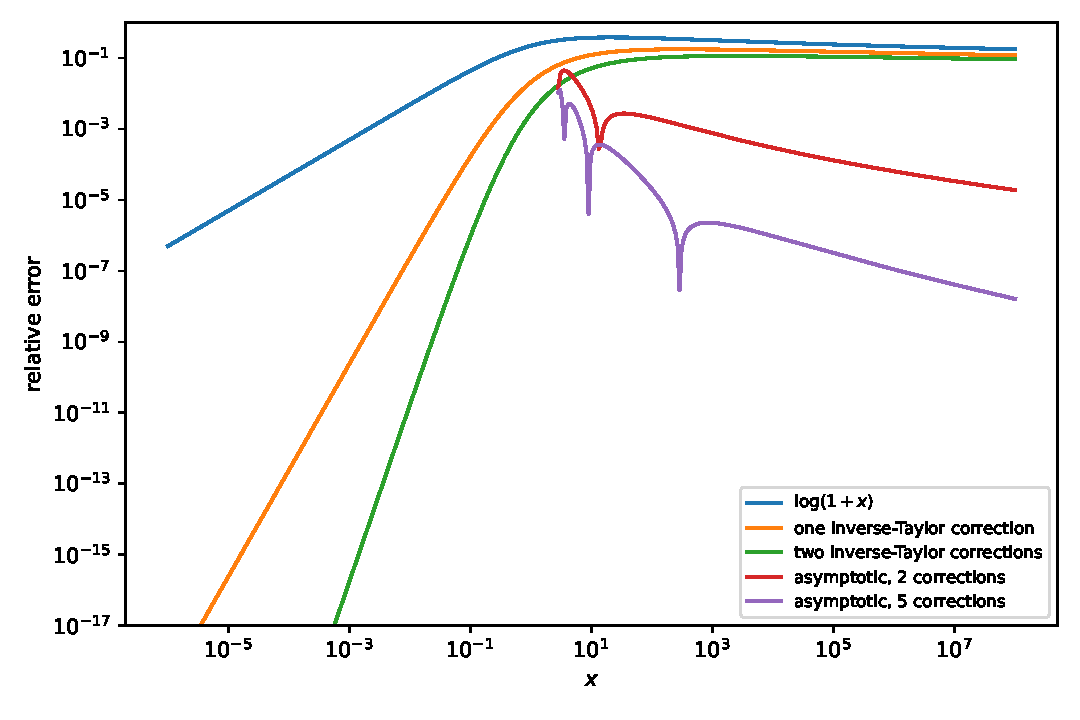
\includegraphics[width=0.82\textwidth]{w0_approximation_errors.pdf}
\caption{Relative errors of several inexpensive approximations to \(W_0\).
Inverse-Taylor correction rapidly improves the global seed \(\log(1+x)\),
while logarithmic asymptotics dominate for large arguments.}
\label{fig:w0approxerrors}
\end{figure}

\begin{figure}[htbp]
\centering
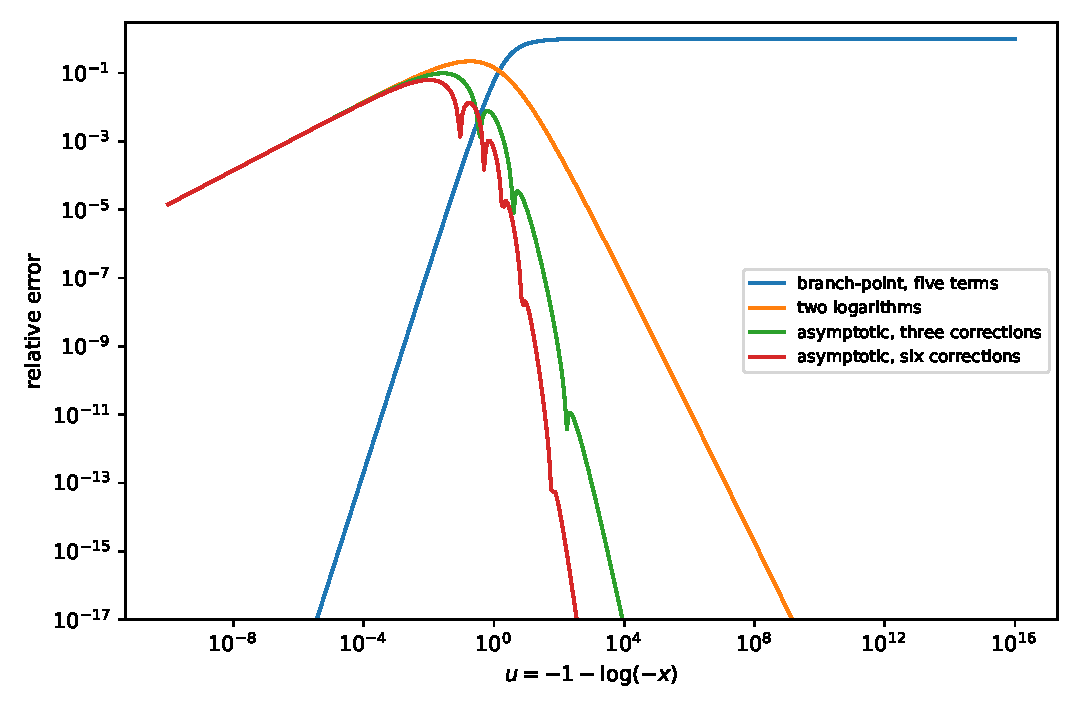
\includegraphics[width=0.82\textwidth]{wm1_approximation_errors.pdf}
\caption{Relative errors on \(W_{-1}\), parametrized by
\(q=-1-\log(-x)\).  The branch-point and logarithmic expansions cover
opposite ends of the interval.}
\label{fig:wm1approxerrors}
\end{figure}

\section{What the approximation literature contributes}
The papers in the supplied archive pursue complementary objectives.

\begin{longtable}{@{}>{\raggedright\arraybackslash}p{0.20\textwidth}>{\raggedright\arraybackslash}p{0.19\textwidth}>{\raggedright\arraybackslash}p{0.51\textwidth}@{}}
\caption{Selected approximation sources in the archive.}\label{tab:approxsources}\\
\toprule
source & branches & main emphasis \\
\midrule
\endfirsthead
\toprule
source & branches & main emphasis \\
\midrule
\endhead
Barry et al. \cite{Barry2000}
& \(W_0,W_{-1}\)
& Explicit piecewise real approximations designed for direct use or as
iteration seeds; the paper is notable for treating the lower branch explicitly.\\

Iacono--Boyd \cite{IaconoBoyd2017}
& \(W_0\)
& Global analytic and spectral approximations, tight large-argument bounds,
and an efficient refinement scheme for the principal branch.\\

Howard \cite{Howard2022}
& mainly \(W_0\)
& Geometric and two-point spline constructions whose accuracy can be increased
systematically on positive and negative compact intervals.\\

Howard \cite{Howard2025}
& \(W_0,W_{-1}\)
& Generic Schr\"oder-type inverse series built from an arbitrary initial
approximating function, with branch-specific convergence conditions.\\

L\'{o}czi \cite{Loczi2022}
& \(W_0,W_{-1}\)
& Monotone logarithmic recursion, explicit starting values, and rigorous
a-priori iteration counts for guaranteed high precision.\\

Corcino--Corcino--Mez\H{o} \cite{Corcino2018}
& \(W_0\)
& C-fractions and associated continued fractions, together with numerical
study of their convergents.\\
\bottomrule
\end{longtable}

The formulas developed in this monograph are deliberately transparent and
proof-oriented.  For production code requiring a certified number of hundreds
or thousands of digits, the sharper enclosures and implementation details in
\cite{Loczi2022} are particularly relevant.

\chapter{Branch-aware numerical evaluation}\label{chap:numerics}

\section{Why solve the logarithmic equation?}
Direct Newton iteration for
\[
             f(y)=y\e^y-x
\]
can overflow when \(y\) is large and can underflow when \(x\) is extremely
small on \(W_{-1}\).  On a correctly selected real branch, \(x/y>0\), and the
equivalent logarithmic equation is
\begin{equation}\label{eq:logroot}
        g_x(y)=y+\log\abs y-\log\abs x=0.
\end{equation}
Its derivatives are
\[
        g_x'(y)=1+\frac1y,
        \qquad
        g_x''(y)=-\frac1{y^2}<0.
\]
Newton's method becomes
\begin{equation}\label{eq:lognewton}
 \boxed{
 y_{n+1}=\frac{y_n}{1+y_n}
       \left(1+\log\frac{x}{y_n}\right).
 }
\end{equation}
The ratio \(x/y_n\) is positive, so the ordinary real logarithm is used on
both negative branches as well as on the positive axis.

\section{Global convergence from elementary starts}
The concavity of \(g_x\) gives a clean convergence proof.

\begin{theorem}[Branch-aware logarithmic Newton iteration]
\label{thm:globalnewton}
Assume \(x\ne-1/\e,0\), and use iteration \eqref{eq:lognewton}.

\begin{enumerate}[label=(\alph*)]
\item If \(x>0\), set \(y_0=\log(1+x)\).  Then
\[
       0<y_1\le W_0(x),
       \qquad y_n\uparrow W_0(x)\quad(n\ge1).
\]

\item If \(-1/\e<x<0\) and the desired branch is \(W_0\), set \(y_0=x\).
Then
\[
       W_0(x)\le y_{n+1}<y_n<0,
       \qquad y_n\downarrow W_0(x).
\]

\item If \(-1/\e<x<0\) and the desired branch is \(W_{-1}\), let
\(T=\log(1/(-x))\) and set \(y_0=-T-\log T\).  Then
\[
       y_1\le W_{-1}(x)<y_0<-1,
       \qquad y_n\uparrow W_{-1}(x)\quad(n\ge1).
\]
\end{enumerate}
\end{theorem}

\begin{proof}
We use the elementary tangent geometry of a concave function.  If a concave
increasing function has a zero \(r\), a Newton step from a point to the right
of \(r\) lands at or to the left of \(r\); subsequent Newton steps from the
left increase and remain at or to the left of \(r\).  If the function is
concave and decreasing, a Newton step from the right remains to the right and
moves left.  These statements follow directly from the fact that the tangent
to a concave graph lies above the graph.

For \(x>0\), \(g_x\) is increasing and concave on \((0,\infty)\).
The bound \(W_0(x)\le\log(1+x)=y_0\) places the start to the right of the
root.  Also \(x>\log(1+x)\), so the explicit formula
\eqref{eq:lognewton} gives \(y_1>0\).  The tangent argument proves the stated
bracketing and monotone convergence.

On \((-1,0)\), \(g_x'(y)<0\), so \(g_x\) is decreasing and concave.  The
bound \(W_0(x)\le x=y_0\) places the start to the right of the root.  Each
Newton step moves left without crossing the root.  The monotone sequence has a
limit, and continuity of the Newton map identifies it as the unique zero in
\((-1,0)\).

For the lower branch, \(g_x\) is increasing and concave on
\(( -\infty,-1)\).  If \(r=W_{-1}(x)=-u\), then
\(u=T+\log u>T+\log T\), hence
\(r<-T-\log T=y_0\).  Thus the start is to the right of the root.  The first
Newton step lands at or to its left and therefore remains below \(-1\).
Subsequent steps increase without crossing the root.  Their limit must be the
unique zero on \(( -\infty,-1)\).
\end{proof}

This theorem uses especially simple starts.  L\'{o}czi's analysis
\cite{Loczi2022} supplies sharper piecewise starts and explicit uniform bounds
on the number of iterations.

\section[Quadratic convergence near the branch point]{Quadratic convergence and its deterioration at the branch point}
Let \(r=W_k(x)\ne-1\) and \(e_n=y_n-r\).  The standard Newton expansion gives
\begin{equation}\label{eq:newtonerror}
 e_{n+1}=-\frac{1}{2r(r+1)}e_n^2+\bigO(e_n^3).
\end{equation}

\begin{proof}
For Newton's method applied to a twice differentiable function with a simple
root,
\[
 e_{n+1}=\frac{g''(r)}{2g'(r)}e_n^2+\bigO(e_n^3).
\]
Here \(g''(r)=-1/r^2\) and
\(g'(r)=(r+1)/r\), giving \eqref{eq:newtonerror}.
\end{proof}

The coefficient becomes unbounded as \(r\to-1\).  This is another expression
of the square-root conditioning.  A branch-point series should therefore be
used to obtain a close initial value before Newton or Halley refinement.

\section{Halley's cubic iteration}
Halley's method applied to \(f(y)=y\e^y-x\) is
\begin{equation}\label{eq:halley}
 y_{n+1}=y_n-
 \frac{y_n\e^{y_n}-x}
 {\e^{y_n}(1+y_n)-
  \dfrac{(y_n+2)(y_n\e^{y_n}-x)}{2(1+y_n)}}.
\end{equation}
At a simple root \(r\),
\begin{equation}\label{eq:halleyerror}
 e_{n+1}=\frac{r^2+4r+6}{12(r+1)^2}e_n^3
 +\bigO(e_n^4).
\end{equation}

\begin{proof}
The general Halley formula is
\[
 y_{n+1}=y_n-
 \frac{2ff'}{2(f')^2-ff''}.
\]
Substituting
\(f=y\e^y-x\), \(f'=\e^y(1+y)\), and
\(f''=\e^y(y+2)\) gives \eqref{eq:halley}.  Taylor expansion of the general
formula at a simple root gives the cubic coefficient
\[
 \frac{f''(r)^2}{4f'(r)^2}-\frac{f'''(r)}{6f'(r)}.
\]
Since \(f'''(r)=\e^r(r+3)\), simplification yields
\((r^2+4r+6)/(12(r+1)^2)\).
\end{proof}

Halley usually reaches machine precision in fewer iterations than Newton after
a good seed.  It is not a substitute for correct branch selection, and its
denominators are again sensitive near \(r=-1\).

\section{A practical real-branch algorithm}
The following procedure combines the theory developed above.  Thresholds are
engineering choices rather than mathematical constants and may be tuned for a
particular floating-point format.

\begin{algorithm}[Piecewise real Lambert \(W\) evaluation]
\label{alg:realW}
Given a real argument \(x\) and branch \(k\in\{0,-1\}\):
\begin{enumerate}[label=\arabic*.]
\item Validate the domain.  For \(k=0\), require \(x\ge-1/\e\).  For
\(k=-1\), require \(-1/\e\le x<0\).
\item Return exact endpoint values when \(x=0\) on \(W_0\) or
\(x=-1/\e\) on either branch.
\item Compute \(d=1+\e x\).  If \(d\) is small, initialize with five to ten
terms of the Puiseux series, using \(p>0\) for \(W_0\) and \(-p\) for
\(W_{-1}\).
\item Otherwise, initialize as follows:
\begin{itemize}
\item \(W_0(x)\), \(x<0\): \(y=x\);
\item \(W_0(x)\), moderate \(x>0\): \(y=\log(1+x)\);
\item \(W_0(x)\), large \(x\): a few terms of \eqref{eq:w0asymp};
\item \(W_{-1}(x)\), moderate \(x\): \(y=-T-\log T\);
\item \(W_{-1}(x)\), very small \(-x\): a few terms of
\eqref{eq:wm1asymp}.
\end{itemize}
\item Refine with logarithmic Newton or Halley iteration.  Stop only when both
the proposed correction and a scaled residual satisfy the requested tolerance.
\item Verify that the final value remains in the required range:
\(y\ge-1\) for \(W_0\), and \(y\le-1\) for \(W_{-1}\).
\end{enumerate}
\end{algorithm}

\section{Floating-point details that matter}
\begin{enumerate}[label=\arabic*.]
\item Use \texttt{log1p(x)} for \(\log(1+x)\) when \(x\) is small.
\item Near the branch point, compute \(1+\e x\) with fused operations when
available, or accept the offset \(x+1/\e\) directly.
\item On \(W_{-1}\), an input may be naturally supplied as
\(x=-\e^{-T}\).  Carrying \(T\) instead of forming \(x\) prevents underflow.
\item Evaluate \(\log(x/y)\), not \(\log\abs{x}-\log\abs{y}\), when \(x\) and \(y\)
are both negative and their ratio is representable.
\item A small residual near \(-1/\e\) is not sufficient by itself; combine it
with the condition number or with a bracket as in
\eqref{eq:residualbound}--\eqref{eq:logresidualbound}.
\end{enumerate}

\begin{table}[htbp]
\centering
\caption{Iterations of the logarithmic Newton method with the elementary
branch-aware starts of \Cref{thm:globalnewton}.}
\label{tab:iterations}
\begin{tabular}{@{}rcrr@{}}
\toprule
argument & branch & steps for $10^{-15}$ & final absolute error \\
\midrule
$10$ & $W_0$ & 4 & $1.627e-19$ \\
$-0.1$ & $W_0$ & 4 & $6.044e-21$ \\
$-0.1$ & $W_{-1}$ & 4 & $1.28e-24$ \\
$-1/e+10^{-8}$ & $W_{-1}$ & 16 & $1.483e-21$ \\
$-10^{-30}$ & $W_{-1}$ & 2 & $1.108e-17$ \\
\bottomrule
\end{tabular}

\end{table}

\begin{figure}[htbp]
\centering
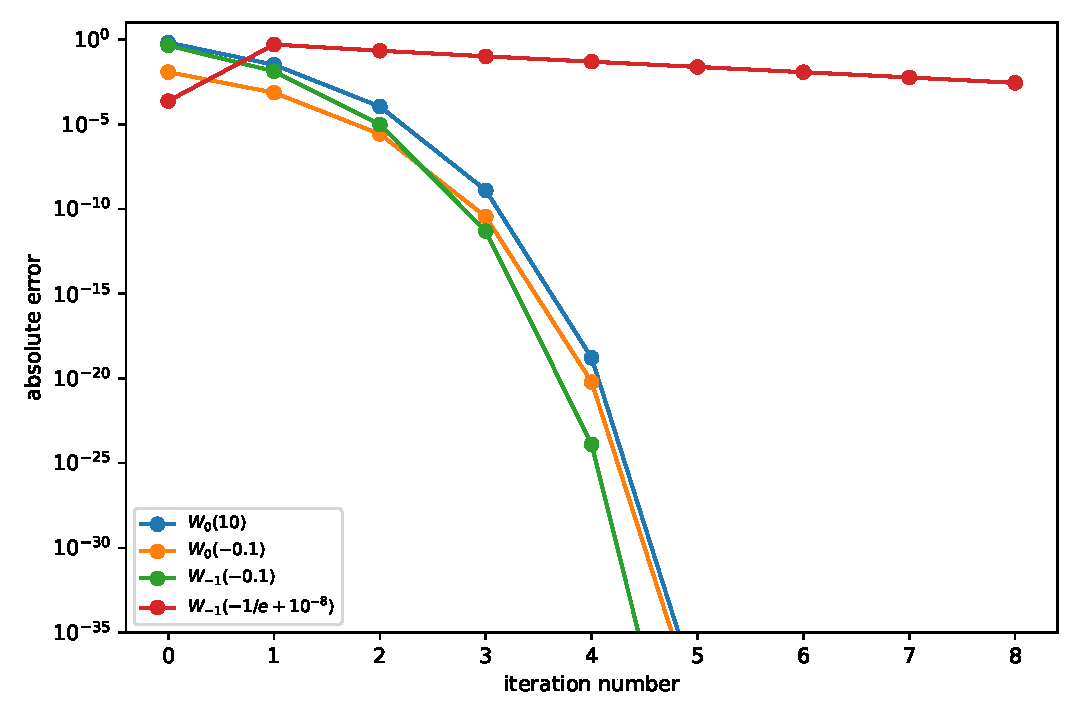
\includegraphics[width=0.82\textwidth]{log_newton_convergence.pdf}
\caption{Absolute error of logarithmic Newton iteration on representative
arguments.  Convergence remains quadratic away from the coalescing root at
\(-1/\e\).}
\label{fig:newtonconvergence}
\end{figure}

\part{Applications}

\chapter{Rooted labeled trees and the tree function}\label{chap:trees}

\section{Cayley's formula}
The appearance of \(n^{n-1}\) in \eqref{eq:treeseries} is not accidental.
We begin with the classical enumeration theorem.

\begin{theorem}[Cayley]
There are \(n^{n-2}\) trees on a fixed set of \(n\ge2\) labeled vertices.
Consequently, there are \(n^{n-1}\) rooted labeled trees on those vertices.
\end{theorem}

\begin{proof}
A Pr\"ufer code associates a sequence of length \(n-2\) over the alphabet
\(\{1,\ldots,n\}\) with each labeled tree.  Given a tree, repeatedly remove
the smallest-labeled leaf and record its unique neighbor.  After \(n-2\)
removals, two vertices remain; the recorded labels form the code.

Conversely, given a sequence \((a_1,\ldots,a_{n-2})\), at each stage connect
the smallest label not appearing in the remaining sequence to the first
remaining entry, then delete that entry and the chosen label.  Finally connect
the last two labels.  This reconstructs a tree and reverses the encoding.
Thus trees are in bijection with the \(n^{n-2}\) sequences.  Choosing one of
the \(n\) vertices as a root multiplies the count by \(n\).
\end{proof}

\section{Why the functional equation is \texorpdfstring{\(T=z\e^T\)}{T=z exp(T)}}
Let
\[
       T(z)=\sum_{n\ge1}t_n\frac{z^n}{n!}
\]
be the exponential generating function for rooted labeled trees.  Remove the
root.  What remains is an unordered set of rooted labeled trees, one for each
neighbor of the old root.  In labeled enumeration, an unordered set of
objects with exponential generating function \(T\) has generating function
\(\e^T\); the extra root contributes a factor \(z\).  Hence
\begin{equation}\label{eq:treefunctional}
               T(z)=z\e^{T(z)}.
\end{equation}

For completeness, the coefficient mechanism behind the exponential is this:
choosing \(j\) unordered components contributes \(T(z)^j/j!\), and summing
over \(j\ge0\) gives \(\sum T^j/j!=\e^T\).  The labels are distributed among
the components by the multinomial coefficients already built into
exponential generating functions.

Equation \eqref{eq:treefunctional} is equivalent to
\[
        -T(z)\e^{-T(z)}=-z,
\]

after multiplying by \(-1\).  Therefore
\begin{equation}\label{eq:treeW}
               T(z)=-W_0(-z).
\end{equation}
Lagrange inversion now gives
\[
        t_n=n^{n-1},
\]
recovering the rooted form of Cayley's formula analytically.

\section{Forests and powers of \texorpdfstring{\(W\)}{W}}
An unordered forest of \(m\) rooted labeled trees has exponential generating
function \(T(z)^m/m!\).  Applying Lagrange inversion to
\(T=z\e^T\) gives
\[
 [z^n]T(z)^m
 =\frac mn[t^{n-m}]\e^{nt}
 =\frac mn\frac{n^{n-m}}{(n-m)!}.
\]
Thus the number of forests on \(n\) labeled vertices with exactly \(m\)
rooted components is
\begin{equation}\label{eq:forestcount}
 n!\,[z^n]\frac{T(z)^m}{m!}
 =\binom{n}{m}m n^{n-m-1}.
\end{equation}
This formula can also be read as: choose the \(m\) roots, then form a forest
oriented toward them.  It illustrates why the power series
\eqref{eq:wpowerseries} is combinatorially meaningful rather than merely a
formal curiosity.

\section{The singularity and coefficient growth}
The dominant positive singularity of \(T\) is \(z=1/\e\).  Substituting
\(x=-z\) in the branch-point expansion gives, with
\(p=\sqrt{2(1-\e z)}\),
\begin{equation}\label{eq:Tsingular}
 T(z)=1-p+\frac13p^2-\frac{11}{72}p^3+\cdots.
\end{equation}
The square-root singularity is responsible for the power \(n^{-3/2}\) in the
asymptotic size of the exponential-generating-function coefficients.  Directly
from Stirling's formula,
\begin{equation}\label{eq:treeasymp}
       \frac{n^{n-1}}{n!}
       \sim\frac{\e^n}{\sqrt{2\pi}\,n^{3/2}}.
\end{equation}
Thus the geometry of the inverse at \(-1/\e\), the convergence radius
\(1/\e\), and the asymptotic enumeration of trees are three views of the same
phenomenon.

\chapter{Delay equations and exponential dynamics}\label{chap:delays}

\section{A scalar delay differential equation}
Consider
\begin{equation}\label{eq:simpleDDE}
             y'(t)=a\,y(t-\tau),
             \qquad \tau>0.
\end{equation}
Looking for exponential modes \(y(t)=\e^{\lambda t}\) gives
\[
       \lambda\e^{\lambda t}
       =a\e^{\lambda(t-\tau)},
       \qquad
       \lambda\e^{\lambda\tau}=a.
\]
Multiplying by \(\tau\),
\begin{equation}\label{eq:DDEspectrum}
       \lambda_k=\frac1\tau W_k(a\tau),
       \qquad k\in\mathbb Z.
\end{equation}
A delay equation has infinitely many characteristic exponents because \(W\)
has infinitely many complex branches.  The complex branch structure is not an
ornament here; it is the spectrum.

\section{The affine linear delay equation}
The more general equation
\begin{equation}\label{eq:affineDDE}
       y'(t)=\alpha y(t)+\beta y(t-\tau)
\end{equation}
has characteristic equation
\[
       \lambda=\alpha+\beta\e^{-\lambda\tau}.
\]
Let \(u=(\lambda-\alpha)\tau\).  Then
\[
       u\e^u=\beta\tau\e^{-\alpha\tau},
\]
so
\begin{equation}\label{eq:affineDDEspectrum}
       \lambda_k=\alpha+\frac1\tau
       W_k\!\left(\beta\tau\e^{-\alpha\tau}\right).
\end{equation}
Every mode follows by a one-line reduction to the inverse relation.
Determining stability still requires examining the real parts of all relevant
branches.

\section{How the two real branches enter a delay spectrum}
For the negative-feedback equation
\[
             y'(t)=-a y(t-\tau),
             \qquad a>0,
\]
we have \(\lambda_k=\tau^{-1}W_k(-a\tau)\).  If
\(0<a\tau<1/\e\), two characteristic exponents are real:
\[
       \lambda_0=\frac1\tau W_0(-a\tau),
       \qquad
       \lambda_{-1}=\frac1\tau W_{-1}(-a\tau).
\]
The \(W_{-1}\) mode is more negative and therefore decays faster.  When
\(a\tau>1/\e\), these two real modes merge and continue as a complex-conjugate
pair on adjacent sheets.

The loss of stability occurs later.  Put \(\lambda=\ii\omega\) in
\(\lambda=-a\e^{-\lambda\tau}\).  Taking absolute values gives
\(\omega=a\).  Matching arguments at the first crossing gives
\[
       \frac\pi2=\pi-a\tau,
       \qquad a\tau=\frac\pi2.
\]
Thus the branch point \(a\tau=1/\e\) marks the transition from real to
oscillatory dominant modes, while \(a\tau=\pi/2\) marks the first imaginary-axis
crossing.  These are distinct dynamical events.

\section{Falling with linear drag: an inversion in time}
Let an object start from rest and approach terminal speed \(v_\infty\) with
linear-drag time scale \(1/k\).  Its distance after time \(t\) is
\[
 s(t)=v_\infty t-\frac{v_\infty}{k}(1-\e^{-kt}).
\]
Set \(u=kt\) and \(D=ks/v_\infty\).  Then
\[
       D=u-1+\e^{-u}.
\]
Writing \(c=D+1\) and \(v=c-u\), we obtain
\[
       v\e^{-v}=\e^{-c},
       \qquad
       -v=W_k(-\e^{-c}),
\]
so
\begin{equation}\label{eq:fallingtime}
       t=\frac{D+1+W_k(-\e^{-D-1})}{k}.
\end{equation}
For \(D>0\), the principal branch gives the positive physical time.  The
lower branch produces a nonpositive algebraic solution and is rejected by the
initial-value problem.  At \(D=0\), the two branches coalesce and give
\(t=0\).

\chapter{Kinetics, epidemics, and ecological models}\label{chap:biology}

\section{A universal logarithm-plus-linear equation}
Many integrated rate laws reduce to
\begin{equation}\label{eq:xalogx}
              x+a\log x=b,
              \qquad x>0,
\end{equation}
where \(a\ne0\).  Dividing by \(a\) and exponentiating gives
\[
       x\e^{x/a}=\e^{b/a},
\]
so
\begin{equation}\label{eq:xalogxsolution}
       x=aW_k\!\left(\frac1a\e^{b/a}\right).
\end{equation}
The branch and even the sign of the argument depend on \(a\).  For \(a>0\)
the argument is positive and only \(W_0\) is real; for \(a<0\), two real
solutions may occur.

\section{Integrated Michaelis--Menten kinetics}
Let \(S(t)>0\) be substrate concentration and suppose
\begin{equation}\label{eq:MM}
       \frac{\dd S}{\dd t}
       =-\frac{V_{\max}S}{K_M+S},
       \qquad S(0)=S_0>0.
\end{equation}
Separating variables gives
\[
       \left(1+\frac{K_M}{S}\right)\dd S=-V_{\max}\dd t,
\]
and hence
\[
       S+K_M\log S
       =S_0+K_M\log S_0-V_{\max}t.
\]
Put \(s=S/K_M\), \(s_0=S_0/K_M\).  Constants involving
\(\log K_M\) cancel, leaving
\[
       s+\log s=s_0+\log s_0-\frac{V_{\max}}{K_M}t.
\]
Exponentiation yields
\[
       s\e^s=s_0\exp\left(s_0-\frac{V_{\max}}{K_M}t\right),
\]
so the exact solution is
\begin{equation}\label{eq:MMsolution}
 S(t)=K_M W_0\!\left(
   \frac{S_0}{K_M}
   \exp\left(\frac{S_0-V_{\max}t}{K_M}\right)
 \right).
\end{equation}
The argument is positive, so the principal branch is forced by positivity.
This example, and more complicated modified rate laws, are developed in the
biochemical review by Goli\v{c}nik \cite{Golicnik2012}.

\section{The final-size equation of an SIR epidemic}
In normalized SIR variables, let \(s+i+r=1\) and
\[
       \dot s=-\mathcal R_0 s i,
       \qquad
       \dot r=i.
\]
Eliminating time gives
\[
       \frac{\dd s}{\dd r}=-\mathcal R_0s,
       \qquad
       \log\frac{s}{s_0}=-\mathcal R_0(r-r_0).
\]
At the end of the epidemic, \(i_\infty=0\) and
\(r_\infty=1-s_\infty\).  Therefore
\[
 s_\infty
 =s_0\exp\{-\mathcal R_0(1-s_\infty-r_0)\}.
\]
Multiplication by \(-\mathcal R_0\e^{-\mathcal R_0s_\infty}\) gives
\begin{equation}\label{eq:SIRfinal}
 s_\infty=-\frac1{\mathcal R_0}
 W_k\!\left(
  -\mathcal R_0s_0\e^{-\mathcal R_0(1-r_0)}
 \right).
\end{equation}

The limiting idealization \(s_0=1\), \(r_0=0\) makes branch selection
particularly instructive:
\[
 s_\infty=-\frac1{\mathcal R_0}
 W_k(-\mathcal R_0\e^{-\mathcal R_0}).
\]
If \(\mathcal R_0>1\), then
\(W_{-1}(-\mathcal R_0\e^{-\mathcal R_0})=-\mathcal R_0\), which gives the
trivial solution \(s_\infty=1\).  The physically relevant macroscopic
outbreak is furnished by \(W_0\), giving \(s_\infty<1/\mathcal R_0\).  If
\(0<\mathcal R_0<1\), the value \(-\mathcal R_0\) belongs instead to the
principal range, so \(W_0\) gives the no-outbreak solution and the lower branch
would give \(s_\infty>1\), which is inadmissible.  The branch switch mirrors
the epidemic threshold.

Lambert \(W\) appears in many related ecological and evolutionary problems,
including marginal-value optimization, population growth rates, mate search,
and fertilization kinetics; Lehtonen gives a broad model-centered survey
\cite{Lehtonen2016}.

\chapter{Diode circuits and physical transcendental equations}
\label{chap:physics}

\section{The generalized diode equation}
For a diode with saturation current \(I_s\), series resistance \(R\), applied
voltage \(V\), and thermal-voltage factor \(a=nV_T>0\), the Shockley law with
series resistance is
\begin{equation}\label{eq:diode}
       I=I_s\left(\exp\frac{V-RI}{a}-1\right).
\end{equation}
Set \(J=I+I_s\).  Since \(I=J-I_s\),
\[
 J=I_s\exp\left(\frac{V+RI_s-RJ}{a}\right).
\]
Thus
\[
       \frac{RJ}{a}\exp\left(\frac{RJ}{a}\right)
       =\frac{RI_s}{a}
        \exp\left(\frac{V+RI_s}{a}\right),
\]
and
\begin{equation}\label{eq:diodesolution}
 I=\frac{a}{R}W_0\!\left(
    \frac{RI_s}{a}\exp\frac{V+RI_s}{a}
   \right)-I_s.
\end{equation}
The argument is positive, so the current is single-valued on \(W_0\).  This
closed form creates a smooth analytical bridge between exponential diode
behavior and the resistor-dominated regime.  Banwell uses it as the basis for
broader bipolar-transistor circuit analysis \cite{Banwell2000}.

\section{Wien's displacement equation and a discarded branch}
The maximum of the wavelength form of Planck's blackbody spectrum leads to
\begin{equation}\label{eq:wien}
             5(1-\e^{-x})=x.
\end{equation}
Let \(y=x-5\).  Then
\[
       y\e^y=-5\e^{-5},
\]
so
\begin{equation}\label{eq:wiensolution}
       x=5+W_k(-5\e^{-5}).
\end{equation}
Because the argument lies in \((-1/\e,0)\), there are two real branch values.
The lower branch is exact:
\[
       W_{-1}(-5\e^{-5})=-5,
\]
which gives \(x=0\), a boundary root introduced by the algebraic stationarity
equation.  The nonzero physical maximum is
\[
       x=5+W_0(-5\e^{-5})
       =4.965114231744\ldots.
\]
This is a model example of why both branches must be written down before
physical constraints are imposed.

\section{A generic saturation equation}
Equations of the form
\begin{equation}\label{eq:saturation}
       A(1-\e^{-bx})=cx,
       \qquad A,b,c>0,
\end{equation}
occur in transport, charging, response saturation, and finite-time relaxation.
Put \(d=Ab/c\) and \(u=bx\).  Then
\[
       d(1-\e^{-u})=u.
\]
The same algebra as in the Wien example gives
\begin{equation}\label{eq:saturationsolution}
       u=d+W_k(-d\e^{-d}),
       \qquad
       x=\frac{d+W_k(-d\e^{-d})}{b}.
\end{equation}
One branch always gives the trivial root \(u=0\); depending on whether
\(d>1\), the other branch gives a positive nontrivial response.  The threshold
\(d=1\) is exactly the coalescence point of the two real branches.

\chapter{Prime-number inversion}\label{chap:primes}

\section{Inverting \texorpdfstring{\(y\log y=x\)}{y log y=x}}
The elementary inverse
\[
       y\log y=x
       \quad\Longleftrightarrow\quad
       y=\exp(W_0(x))=\frac{x}{W_0(x)}
\]
turns classical estimates involving \(n\log n\) into estimates involving
\(W\).  This is the basic observation behind Visser's treatment of primes
\cite{Visser2018}.

\begin{theorem}[A Lambert \(W\) upper bound for the prime-counting function]
Assume the classical Rosser inequality \(p_n>n\log n\) for \(n\ge1\).  Then
for \(x\ge0\),
\begin{equation}\label{eq:pibound}
       \pi(x)<\exp(W_0(x))=\frac{x}{W_0(x)},
\end{equation}
with the quotient interpreted by continuity at \(x=0\).
\end{theorem}

\begin{proof}
For \(x<2\), the assertion is checked directly.  For \(x\ge2\), let
\(n=\pi(x)\), so \(p_n\le x\).  The assumed prime bound gives
\[
       x\ge p_n>n\log n.
\]
The function \(y\mapsto y\log y\) is increasing for \(y\ge1\).  Its inverse
at \(x\) is \(\exp(W_0(x))\), so
\(n<\exp(W_0(x))\).  Finally,
\(\exp(W_0(x))=x/W_0(x)\) follows from the defining relation.
\end{proof}

\section{Why the lower branch estimates the \texorpdfstring{\(n\)th}{nth} prime}
The rough relation \(n\approx x/\log x\) is inverted as follows.  Put
\(u=\log x\), so \(x=\e^u\).  Then
\[
       n=\frac{\e^u}{u}
       \quad\Longleftrightarrow\quad
       (-u)\e^{-u}=-\frac1n.
\]
The large solution has \(u>1\), so \(-u<-1\) and the correct branch is
\(W_{-1}\):
\begin{equation}\label{eq:primefirstsurrogate}
       x=-nW_{-1}(-1/n).
\end{equation}
The principal branch would give a small \(u\) and therefore the wrong inverse.

Using known explicit inequalities for \(\pi(x)\), Visser proves, for example,
\begin{equation}\label{eq:pnupper}
       p_n<-nW_{-1}(-1/n),
       \qquad n\ge4.
\end{equation}
The Lambert form cleanly separates the elementary inversion from the
number-theoretic input.

A refined approximation to the prime number theorem is
\[
       n\approx\frac{x}{\log x-1}.
\]
If \(u=\log x-1\), then
\[
       n=\frac{\e^{u+1}}u,
       \qquad
       (-u)\e^{-u}=-\frac\e n,
\]
and hence
\begin{equation}\label{eq:primerefined}
       x\approx-nW_{-1}(-\e/n).
\end{equation}
The first terms of \Cref{thm:wm1asymp} give
\[
 -W_{-1}(-\e/n)
 =\log n+\log\log n-1+\littleo(1),
\]
so the three familiar leading terms of the Ces\`aro--Cipolla expansion appear
automatically.  Higher terms of the Lambert expansion provide a systematic
closed-form refinement, though they do not by themselves replace the deeper
number-theoretic corrections needed for the full asymptotic series of
\(p_n\).

\appendix

\chapter{Formula compendium and coefficient tables}\label{app:formulas}

\section{Real branch summary}
\begin{longtable}{@{}>{\raggedright\arraybackslash}p{0.17\textwidth}>{\raggedright\arraybackslash}p{0.32\textwidth}>{\raggedright\arraybackslash}p{0.38\textwidth}@{}}
\caption{The two real branches at a glance.}\label{tab:branchsummary}\\
\toprule
property & \(W_0\) & \(W_{-1}\) \\
\midrule
\endfirsthead
\toprule
property & \(W_0\) & \(W_{-1}\) \\
\midrule
\endhead
domain
& \([-1/\e,\infty)\)
& \([-1/\e,0)\) \\
range
& \([-1,\infty)\)
& \(( -\infty,-1]\) \\
monotonicity
& increasing
& decreasing \\
curvature
& concave
& convex for \(-2<W<-1\), then concave for \(W<-2\); see
\Cref{chap:calculus} \\
value at branch point
& \(-1\)
& \(-1\) \\
origin behavior
& \(W_0(x)=x-x^2+\cdots\)
& \(W_{-1}(x)\to-\infty\) logarithmically \\
far-end behavior
& \(W_0(x)\sim\log x-\log\log x\)
& \(W_{-1}(x)\sim\log(-x)-\log[-\log(-x)]\) \\
branch-point sign
& \(-1+U(p)\)
& \(-1+U(-p)\) \\
\bottomrule
\end{longtable}

In the curvature row, the argument interval for convexity is
\((-1/\e,-2/\e^2)\), and the interval for concavity is
\((-2/\e^2,0)\).  The compact wording in the table is intended only as a
memory aid.

\section{Derivative polynomials}
The recurrence from \Cref{thm:derivativepolynomials} produces
\[
 W^{(n)}(x)=
 \frac{\e^{-nW(x)}P_n(W(x))}{(1+W(x))^{2n-1}}.
\]
The first eight polynomials are
\begin{align*}
P_1(w)={}&1,\\
P_2(w)={}&-w-2,\\
P_3(w)={}&2w^2+8w+9,\\
P_4(w)={}&-6w^3-36w^2-79w-64,\\
P_5(w)={}&24w^4+192w^3+622w^2+974w+625,\\
P_6(w)={}&-120w^5-1200w^4-5126w^3-11758w^2-14543w-7776,\\
P_7(w)={}&720w^6+8640w^5+45756w^4+137512w^3\\
&\quad+248250w^2+255828w+117649,\\
P_8(w)={}&-5040w^7-70560w^6-445572w^5-1651480w^4\\
&\quad-3892430w^3-5846760w^2-5187775w-2097152.
\end{align*}
The constants \(P_n(0)=(-n)^{n-1}\) reproduce the Maclaurin derivatives.

\section{Branch-point coefficients}
For quick reference, the first coefficients in
\(U(p)=\sum_{n\ge1}c_np^n\) are
\begin{center}
\begin{tabular}{@{}crcr@{}}
\toprule
\(n\) & \(c_n\) & \(n\) & \(c_n\) \\
\midrule
1 & \(1\) & 6 & \(-221/8505\) \\
2 & \(-1/3\) & 7 & \(680863/43545600\) \\
3 & \(11/72\) & 8 & \(-1963/204120\) \\
4 & \(-43/540\) & 9 & \(226287557/37623398400\) \\
5 & \(769/17280\) & 10 & \(-5776369/1515591000\) \\
\bottomrule
\end{tabular}
\end{center}
Use \(W_0=-1+U(p)\) and \(W_{-1}=-1+U(-p)\).

\section{A compact identity list}
For a consistent branch and away from singular points,
\begin{align*}
 W\e^W&=x,\\
 \e^W&=\frac{x}{W},\\
 W&=\log x-\log W,\\
 W'&=\frac{W}{x(1+W)}=\frac{\e^{-W}}{1+W},\\
 xW'&=\frac{W}{1+W},\\
 \frac{\dd}{\dd x}\left(W+\frac12W^2\right)&=\frac{W}{x},\\
 \frac{\dd}{\dd x}\left(\frac{x}{W}\right)&=\frac1{1+W},\\
 \frac{\dd}{\dd x}\log\abs W&=\frac1{x(1+W)}.
\end{align*}
The logarithmic identity must be interpreted with compatible complex branches;
on the real branches it is safest to write
\(W+\log\abs W=\log\abs x\).

\chapter{How the attached archive was used}\label{app:archive}

The supplied archive combines foundational papers, recent approximation work,
application surveys, reference exports, and a computer-algebra notebook.  The
following guide records the role of each item and helps distinguish primary
sources from convenient secondary summaries.

\begingroup
\small
\begin{longtable}{@{}>{\raggedright\arraybackslash}p{0.35\textwidth}>{\raggedright\arraybackslash}p{0.54\textwidth}@{}}
\caption{Guide to the files in the supplied \texttt{Lambert-W.zip}.}
\label{tab:archiveguide}\\
\toprule
file or group & use in this article \\
\midrule
\endfirsthead
\toprule
file or group & use in this article \\
\midrule
\endhead
\nolinkurl{corless1996.pdf};
\nolinkurl{On-the-Lambert-W-Function.pdf}
& Two renderings of the canonical Corless--Gonnet--Hare--Jeffrey--Knuth paper.
They supplied the standard branch notation, complex continuation, derivative
structure, Maclaurin and branch-point series, all-branch asymptotics, symbolic
integration viewpoint, and historical context.\\

\texttt{DLMF\_4.13 Lambert}\newline\texttt{W-Function.pdf}
& Authoritative reference summary for branches, special values, expansions,
integrals, differential identities, and the Wright omega and tree functions.\\

\nolinkurl{barry2000.pdf}
& Early explicit approximations covering the separate real portions of
\(W_0\) and, importantly, \(W_{-1}\).\\

\nolinkurl{chatzigeorgiou2013.pdf}
& The global square-root-plus-linear bounds for \(W_{-1}(-\e^{-1-q})\),
reproved in \Cref{thm:chatzbounds}.\\

\nolinkurl{corcino2018.pdf}
& The Fourier--logarithm integral and the regular and associated continued
fractions for the principal branch.\\

\nolinkurl{iacono2017.pdf}
& Global principal-branch approximations, spectral approximation issues,
large-argument bounds, and efficient iterative refinement.\\

\nolinkurl{10.1016@j.amc.2022.127406.pdf}
& L\'{o}czi's guaranteed high-precision logarithmic recursion, monotone starts,
and explicit convergence estimates for both real branches.\\

\nolinkurl{_Manuscript.pdf_.pdf}
& Howard's geometric and spline-based construction of systematically
improvable approximations, especially for the principal branch.\\

\nolinkurl{appliedmath-05-00066.pdf}
& Howard's 2025 Schr\"oder-type inverse-series framework for both real
branches.  It motivated the branch-neutral inverse-Taylor treatment in
\Cref{sec:schroeder}.\\

\nolinkurl{banwell2000.pdf}
& Exact generalized-diode and bipolar-transistor formulas using \(W\),
represented here by \eqref{eq:diodesolution}.\\

\nolinkurl{10.1016@j.bej.2012.01.010.pdf}
& Goli\v{c}nik's review of biochemical kinetics, including integrated enzyme
rate laws and related transport-limited systems.\\

\nolinkurl{lehtonen2016.pdf}
& Broad ecological and evolutionary survey, including epidemic, population,
optimization, and search models.\\

\nolinkurl{visser2018.pdf}
& Prime-counting and \(n\)th-prime bounds and asymptotics expressed through
\(W_0\) and \(W_{-1}\).\\

\nolinkurl{ProductLog.nb}; \nolinkurl{ProductLog.pdf}
& A Wolfram notebook and rendered output illustrating symbolic identities,
series, and the computer-algebra notation \texttt{ProductLog}.  They were used
as computational cross-checks, not as the source of proofs.\\

\texttt{Lambert W-Function --}\newline\texttt{from Wolfram MathWorld.pdf}
& Secondary reference for historical notes, identities, and special values.\\

\texttt{Lambert W function -}\newline\texttt{Wikipedia.pdf};
\texttt{Lambert W-function.txt}
& Snapshot and source text of a general encyclopedia article.  These were used
only as navigation aids and cross-checks; primary papers and DLMF take
precedence when precision matters.\\
\bottomrule
\end{longtable}
\endgroup

\chapter{Reproducing the numerical experiments}\label{app:repro}

The ZIP accompanying this article contains
\texttt{lambert\_w\_experiments.py}.  The program is deterministic and uses no
random data.  It requires Python 3 together with \texttt{mpmath},
\texttt{numpy}, and \texttt{matplotlib}.  From the article directory, run
\begin{verbatim}
python3 lambert_w_experiments.py
\end{verbatim}
to regenerate the PDF figures and the two small LaTeX tables in the
\texttt{generated} directory.

\section{What the program checks}
The script performs the following independent numerical tasks.
\begin{enumerate}[label=\arabic*.]
\item It evaluates \(W_0\) and \(W_{-1}\) with 50 decimal digits using
\texttt{mpmath} and plots the two real branches.
\item It compares one- and five-term branch-point expansions with high-precision
reference values over many scales of \(1+\e x\).
\item It verifies the condition-number law
\(1/\abs{1+W}\sim1/\sqrt{2(1+\e x)}\).
\item It evaluates the asymptotic polynomials \(P_1,\ldots,P_6\) on both real
branches and plots relative errors.
\item It applies one and two inverse-Taylor corrections to elementary seeds.
\item It tests the monotone logarithmic Newton iteration on positive, negative
principal, lower-branch, and near-branch-point examples.
\item It writes the numerical value and iteration-count tables included in the
book.
\end{enumerate}

The plotted curves are evidence and diagnostics, not substitutes for the
proofs.  In particular, high-precision reference values were used to detect
sign mistakes in the odd powers of the \(W_{-1}\) branch-point series and in
the alternating lower-branch asymptotic corrections.

\section{Compiling the document}
A typical TeX installation can compile the source with
\begin{verbatim}
latexmk -pdf -interaction=nonstopmode lambert_w_monograph.tex
\end{verbatim}
The distributed archive already contains the rendered PDF, all generated
figures, and the generated table fragments, so rerunning the Python program is
optional.

\chapter{Further directions}\label{app:further}

The ordinary Lambert function is the first member of a larger family of
inverse functions.  Equations such as
\[
       x\e^x+r x=a,
\]
products of shifted linear factors times an exponential, and matrix or operator
analogues lead to generalized Lambert functions.  Many techniques in this
article survive: locate critical points of the forward map, choose local
coordinates adapted to those critical points, use Lagrange inversion for local
series, take logarithms for remote asymptotics, and preserve every real inverse
branch during algebraic reduction.

Several questions remain attractive even for the classical function.
Uniform approximations that are simultaneously elementary, branch-aware,
near-minimax, and rigorously certified continue to be refined.  Complex
interval algorithms must manage branch cuts and coalescing roots without losing
correct enclosures.  In applications, an explicit \(W\) formula often exposes
previously hidden multiplicity or threshold behavior; deciding which branch is
physically realized may require stability, initial data, or variational
arguments beyond the algebra itself.

\backmatter

\begin{thebibliography}{99}

\bibitem{Banwell2000}
T.~C. Banwell,
``Bipolar transistor circuit analysis using the Lambert \(W\)-function,''
\emph{IEEE Transactions on Circuits and Systems I}, vol.~47, no.~11,
pp.~1621--1633, 2000.

\bibitem{Barry2000}
D.~A. Barry, J.-Y. Parlange, L.~Li, H.~Prommer, C.~J. Cunningham, and
F.~Stagnitti,
``Analytical approximations for real values of the Lambert \(W\)-function,''
\emph{Mathematics and Computers in Simulation}, vol.~53, pp.~95--103, 2000.

\bibitem{Chatzigeorgiou2013}
I.~Chatzigeorgiou,
``Bounds on the Lambert function and their application to the outage analysis
of user cooperation,''
\emph{IEEE Communications Letters}, vol.~17, no.~8, pp.~1505--1508, 2013.

\bibitem{Corcino2018}
C.~B. Corcino, R.~B. Corcino, and I.~Mez\H{o},
``Continued fraction expansions for the Lambert \(W\) function,''
\emph{Aequationes Mathematicae}, 2018,
doi:10.1007/s00010-018-0559-2.

\bibitem{Corless1996}
R.~M. Corless, G.~H. Gonnet, D.~E.~G. Hare, D.~J. Jeffrey, and D.~E. Knuth,
``On the Lambert \(W\) function,''
\emph{Advances in Computational Mathematics}, vol.~5, pp.~329--359, 1996.

\bibitem{DLMF}
NIST Digital Library of Mathematical Functions,
``Section 4.13: Lambert \(W\)-function,''
F.~W.~J. Olver et al., eds., National Institute of Standards and Technology.

\bibitem{Golicnik2012}
M.~Goli\v{c}nik,
``On the Lambert \(W\) function and its utility in biochemical kinetics,''
\emph{Biochemical Engineering Journal}, vol.~63, pp.~116--123, 2012.

\bibitem{Howard2022}
R.~M. Howard,
``Analytical approximations for the principal branch of the Lambert \(W\)
function,'' manuscript, 2022; copy supplied in the source archive.

\bibitem{Howard2025}
R.~M. Howard,
``On Schr\"oder-type series expansions for the Lambert \(W\) function,''
\emph{AppliedMath}, vol.~5, article 66, 2025,
doi:10.3390/appliedmath5020066.

\bibitem{IaconoBoyd2017}
R.~Iacono and J.~P. Boyd,
``New approximations to the principal real-valued branch of the Lambert
\(W\)-function,''
\emph{Advances in Computational Mathematics}, vol.~43, pp.~1403--1436, 2017.

\bibitem{Lehtonen2016}
J.~Lehtonen,
``The Lambert \(W\) function in ecological and evolutionary models,''
\emph{Methods in Ecology and Evolution}, 2016,
doi:10.1111/2041-210X.12568.

\bibitem{Loczi2022}
L.~L\'{o}czi,
``Guaranteed- and high-precision evaluation of the Lambert \(W\) function,''
\emph{Applied Mathematics and Computation}, vol.~433, article 127406, 2022.

\bibitem{Visser2018}
M.~Visser,
``Primes and the Lambert \(W\) function,''
\emph{Mathematics}, vol.~6, article 56, 2018.

\end{thebibliography}

\end{document}
